\documentclass[10pt,twocolumn,letterpaper]{article}
%\usepackage[review]{cvpr}
%\usepackage[final]{cvpr}
\usepackage[pagenumbers]{cvpr} % To force page numbers, e.g. for an arXiv version


\usepackage[utf8]{inputenc} % allow utf-8 input
\usepackage{url}            % simple URL typesetting
\usepackage{amsfonts}       % blackboard math symbols
\usepackage{nicefrac}       % compact symbols for 1/2, etc.
\usepackage{graphicx}
\usepackage{wrapfig}

% Include other packages here, before hyperref.
\usepackage{graphicx}
\usepackage{amsmath}
\usepackage{amssymb}
\usepackage{booktabs}
\usepackage{placeins}
\usepackage{tabularx}
\usepackage{multirow}
\usepackage{makecell}


%
% --- inline annotations
%
\usepackage[dvipsnames]{xcolor}
\newcommand{\red}[1]{{\color{red}#1}}
\newcommand{\todo}[1]{{\color{red}#1}}
\newcommand{\TODO}[1]{\textbf{\color{red}[TODO: #1]}}
% --- disable by uncommenting  
% \renewcommand{\TODO}[1]{}
% \renewcommand{\todo}[1]{#1}

% It is strongly recommended to use hyperref, especially for the review version.
% hyperref with option pagebackref eases the reviewers' job.
% Please disable hyperref *only* if you encounter grave issues, e.g. with the
% file validation for the camera-ready version.
%
% If you comment hyperref and then uncomment it, you should delete
% ReviewTempalte.aux before re-running LaTeX.
% (Or just hit 'q' on the first LaTeX run, let it finish, and you
%  should be clear).
\definecolor{cvprblue}{rgb}{0.21,0.49,0.74}
\usepackage[pagebackref,breaklinks,colorlinks,citecolor=cvprblue]{hyperref}

\def\confName{ar$\xi$iv}
\def\confYear{2023}

%%% Add PDF metadata to help others organize their library
%%% Once the PDF is generated, you can check the metadata with
%%% $ pdfinfo template.pdf
\hypersetup{
	pdftitle={Beyond the Final Linear Layer},
	pdfauthor={Michael Majurski, David Chapman},
	pdfkeywords={AI,Semi-Supervised,Classification,FixMatch},
}



\begin{document}
	
	% \title{GmmMatch: Enhancing Semi-Supervised Learning with a Generative Gaussian Mixture Model Final Layer}
	% \title{The Use of a Generative Gaussian Mixture Model Final Layer For Enhancing Deep Semi-Supervised Learning}
	% \title{Enhancing Deep Semi-Supervised Learning via a Generative Gaussian Mixture Model Final Layer}
	% \title{Enhancing Semi-Supervised Learning with a Generative Gaussian Mixture Model Final Layer}
	%\title{Training a final activation layer with the method of moments, and its application to semi-supervised learning.}
	\title{A Method of Moments Embedding Constraint for Generative Final Layers}
	
	\author{Michael Majurski\\
		Information Technology Lab, NIST\\
		University of Maryland, Baltimore County\\
		%	100 Bureau Dr. Gaithersburg MD, 20899\\
		{\tt\small michael.majurski@nist.gov}
		% For a paper whose authors are all at the same institution,
		% omit the following lines up until the closing ``}''.
	% Additional authors and addresses can be added with ``\and'',
	% just like the second author.
	% To save space, use either the email address or home page, not both
	\and
	Sumeet Menon\\
	University of Maryland, Baltimore County\\
	{\tt\small sumeet1@umbc.edu}
	\and
	Parniyan Farvardin\\
	University of Miami\\
	{\tt\small pxf291@miami.edu}
	\and
	David Chapman\\
	University of Miami\\
	{\tt\small dchapman@cs.miami.edu}
}

\maketitle




% SCOPE paper review notes that I need to make sure i also address
%3.2- The performance gains obtained with 250 labels and 4000 labels on cifar10 are not significant. A similar case of very limited performance gains on CIFAR100 with 2500 and 4000 labels.

%1. The results are reported only on Cifar-10 and Cifar-100 datasets. Considering that the initial training only is performed for 1024 epochs, is it scalable for larger datasets?


%\begin{abstract}
%	Semi-Supervised Learning (SSL) leverages an abundance of unlabeled data to improve deep learning based model performance under limited training data regimes.
%	This paper presents a novel extension to any image classification architecture which improves accuracy in low-label regimes by enhancing class inlier determination. 
%	We demonstrate our method by extending the FixMatch \cite{sohn2020fixmatch} training scheme with our novel final layers. 
%	We present two semi-parametric final layers of differing complexity (a) the Axis Aligned GMM (AAGMM) layer, and (b) an equal variance version we call KMeans. % of AAGMM we call KMeans.
%	Both layers are integrated into the network architecture as regular fully differentiable modules which are trained via backprop (not Expectation Maximization).
%	Importantly, these novel layers exhibit both discriminative and generative properties, enhancing their capability to characterize inlier data; improving pseudo-labeling performance. 
%	We also introduce and evaluate a series of class-wise embedding constraints based on the Method of Moments (MoM) \cite{pearson1936method} in order to fit the parameters of our semi-parametric latent prior.  
%	These methods match published SOTA 250 label CIFAR-10 \cite{cifar10} accuracy and come close to matching the recently improved SOTA in the 40 label regime without the significant increase in model complexity of other modern SOTA methods \cite{zheng2023simmatchv2}.
%	%Our code is available at: \url{https://github.com/*} % \url{https://github.com/mmajurski/ssl-gmm}
%\end{abstract}

\begin{abstract}
Discriminative deep learning models with a linear+softmax final layer have a problem: the latent space only predicts the conditional probabilities $p(y|x)$ but not the full joint distribution $p(y,x)$, which necessitates a generative approach.
%A problem with deep learning discrimination models with a linear+softmax final layer is that the latent space only predicts the conditional probabilities $p(Y|X)$ but not the full joint distribution $p(Y,X)$ which necessitates a generative approach.
The conditional probability cannot detect outliers, causing sensitivity to them in softmax networks.
%This exacerbates model over-confidence which has been linked to a multitude of problems, ranging from hallucinations, confounding biases, and dependence on large labeled training data.
This exacerbates model over-confidence impacting many problems: from hallucinations, to confounding biases, and dependence on large datasets.
We introduce a novel embedding constraint based on the Method of Moments (MoM).
We investigate the use of polynomial moments ranging from 1st through 4th order hyper-covariance matrices.
Furthermore, we use this embedding constraint to train an Axis-aligned Gaussian Mixture Model (AAGMM) final layer, which learns not only the conditional, but also the joint distribution of the latent space.
%Next, we demonstrate this technique in the problem area of Semi-supervised image classification by extending the well-known FixMatch algorithm.
We demonstrate our approach by extending FixMatch based semi-supervised image classification.
We find our MoM constraint with the AAGMM layer is able to match or improve upon the reported FixMatch accuracy, while also modeling the joint distribution, thereby reducing outlier sensitivity.
%We further include a future work discussion about potential future applications for this layer and embedding constraint, as well as how and why this MoM technique can overcome the theoretical limitations of other existing methods including the approximate KL-divergence constraint of variational autoencoders.
Future work explores potential applications for this layer and embedding constraint, and how/why this MoM technique can overcome theoretical limitations of other existing methods including the approximate KL-divergence constraint of variational autoencoders.
Code is available at: \url{https://github.com/*******} % \url{https://github.com/mmajurski/ssl-gmm}
\end{abstract}


\section{Introduction}

\begin{figure}[ht]
	\centering
	
	\includegraphics[width=0.9\linewidth]{example-image-a}
	\caption{Schematic of the outlier problem, and how generative modeling of the joint probability can improve the situation.} 
	\label{fig:schema}
\end{figure}

%SSL leverages an abundance of unlabeled data to improve deep learning based model performance under limited training data regimes \cite{zhu2022introduction,li2019safe,hady2013semi}.
%Image classification has become a playground for exploring novel SSL ideas.
%The early successes of deep learning based methods relied on large annotated datasets to enable models to learn the relevant features to perform the task, i.e. image classification build on top of ImageNet \cite{deng2009imagenet}.
%With data annotation becoming a significant bottleneck, especially in application domains outside of the standard benchmarks, another learning paradigm was needed.
%
%There are several flavors of SSL.
%Contrastive learning methods leverage the intuition that similar instances should be close in the representation space, while different instances are farther apart \cite{yang2022class,li2021comatch}.
%Consistency regularization borrows the intuition that modified views of the same instance should have similar representations and predictions \cite{sohn2020fixmatch,lee2022contrastive,zhang2021flexmatch,kim2022conmatch}.
%Pseudo-labeling methods like FixMatch \cite{sohn2020fixmatch} fall within the consistency regularization domain.
%
%This work argues that pseudo-labeling methods can be improved with better calibration of the network logits used to filter the pseudo-labels into reliable and unreliable. 
%This is equivalent to improving the accuracy of class inlier determination.
%Neural networks are known to be overconfident in their predictions \cite{wei2022mitigating}, and this affects the pseudo-labeling process. 
%Potentially allowing for the inclusion of more incorrect pseudo-labels any specific logit threshold would otherwise have.
%This work demonstrates the better calibrated replacements for a models final linear layer can improve the final accuracy of pseudo-labeling based SSL algorithms in very label scarce regimes. 

\begin{figure*}[ht]
	\centering
	\subfloat{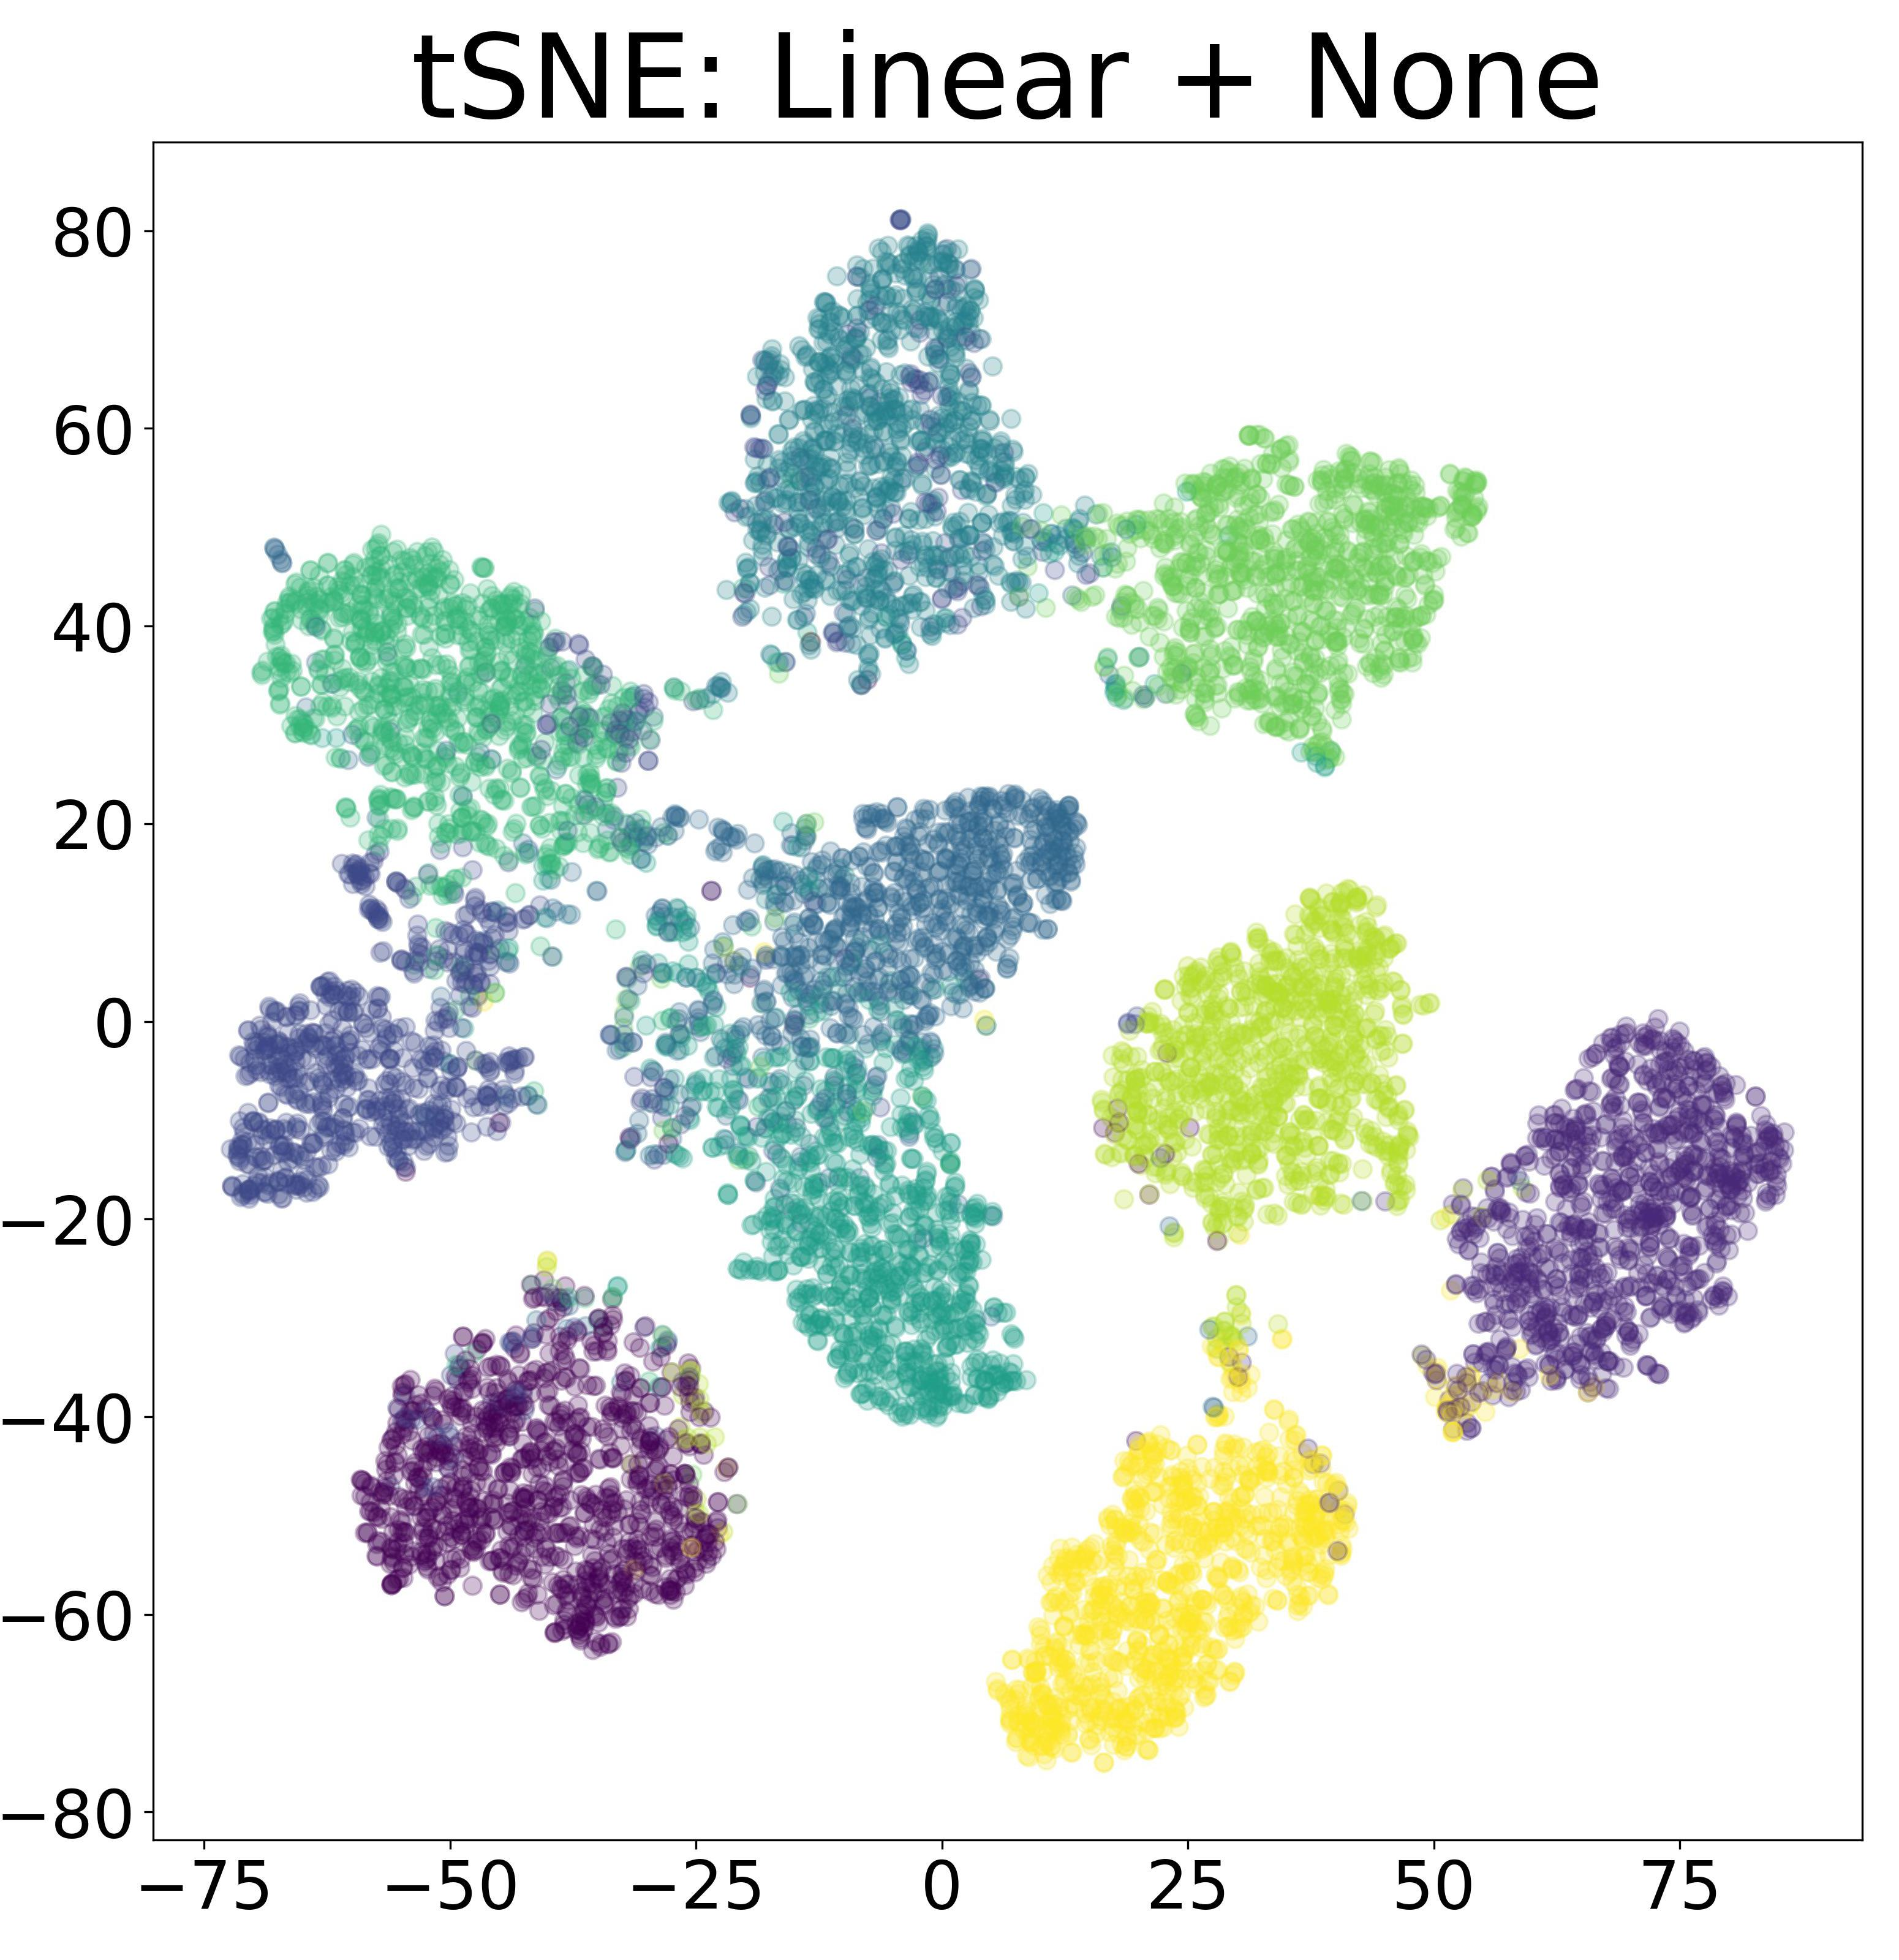
\includegraphics[width=.25\textwidth]{figures/id-00000001-tsne.jpg}}
	\subfloat{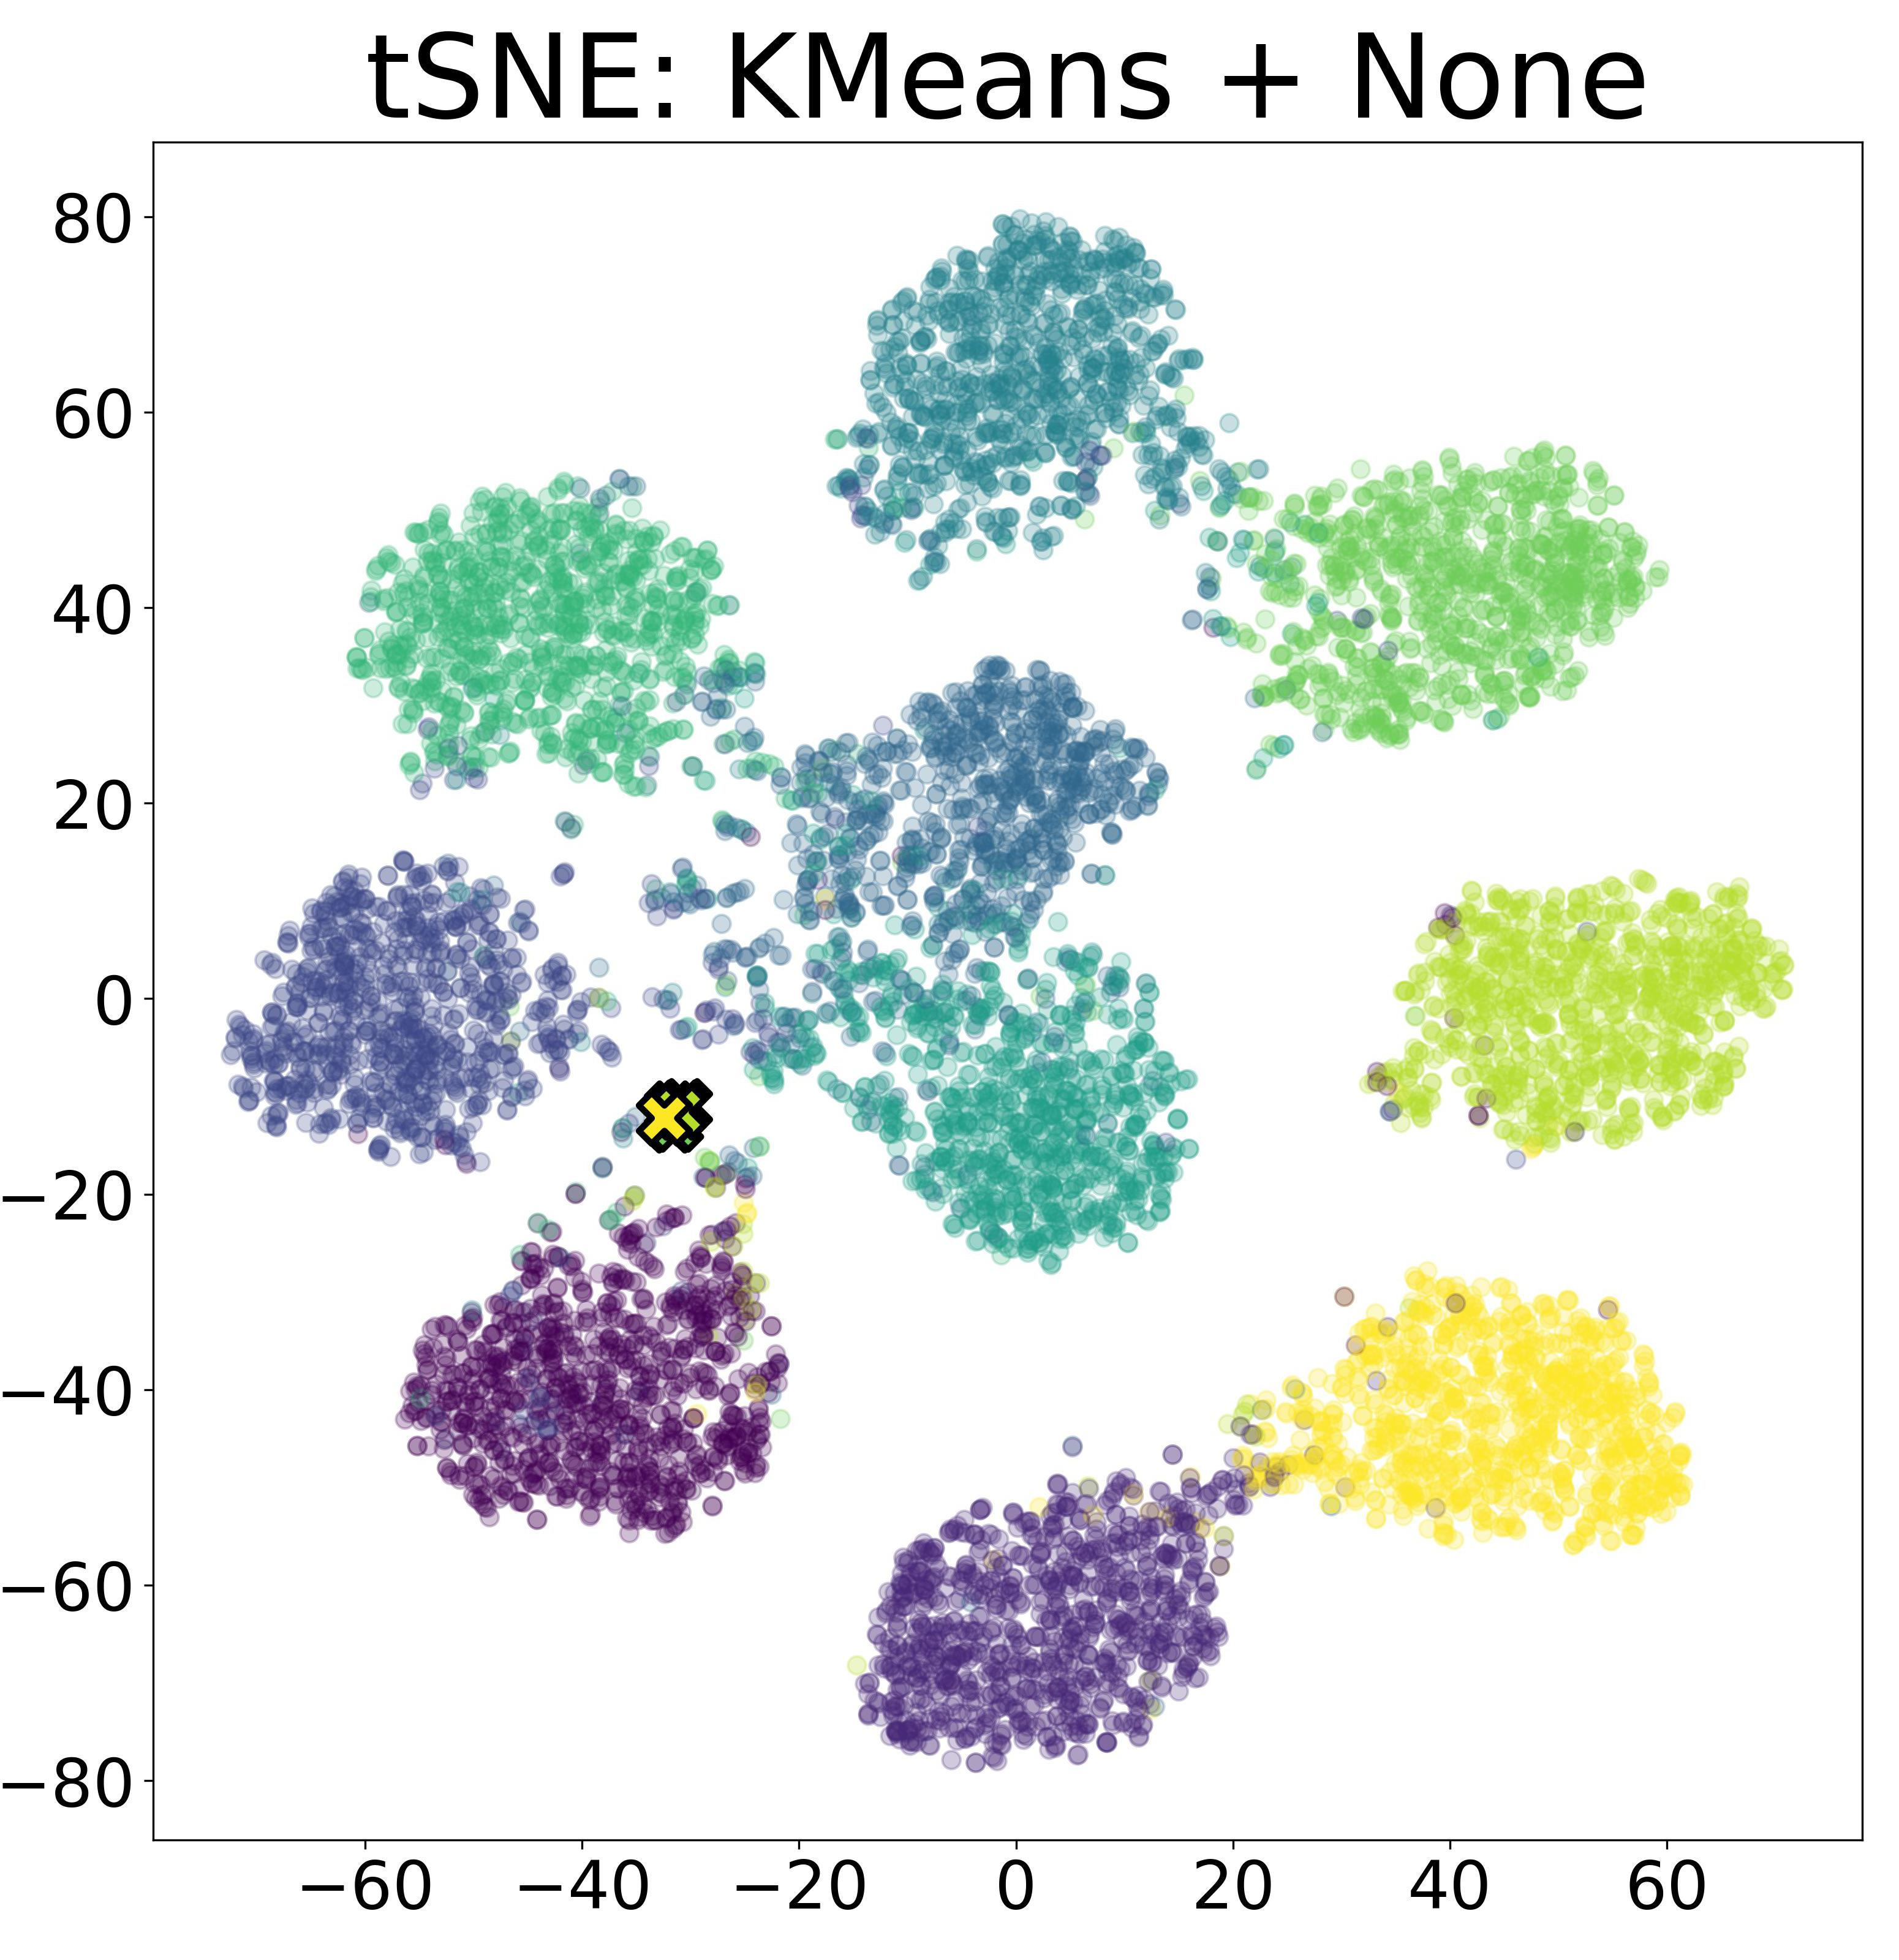
\includegraphics[width=.25\textwidth]{figures/id-00000013-tsne.jpg}}
	\subfloat{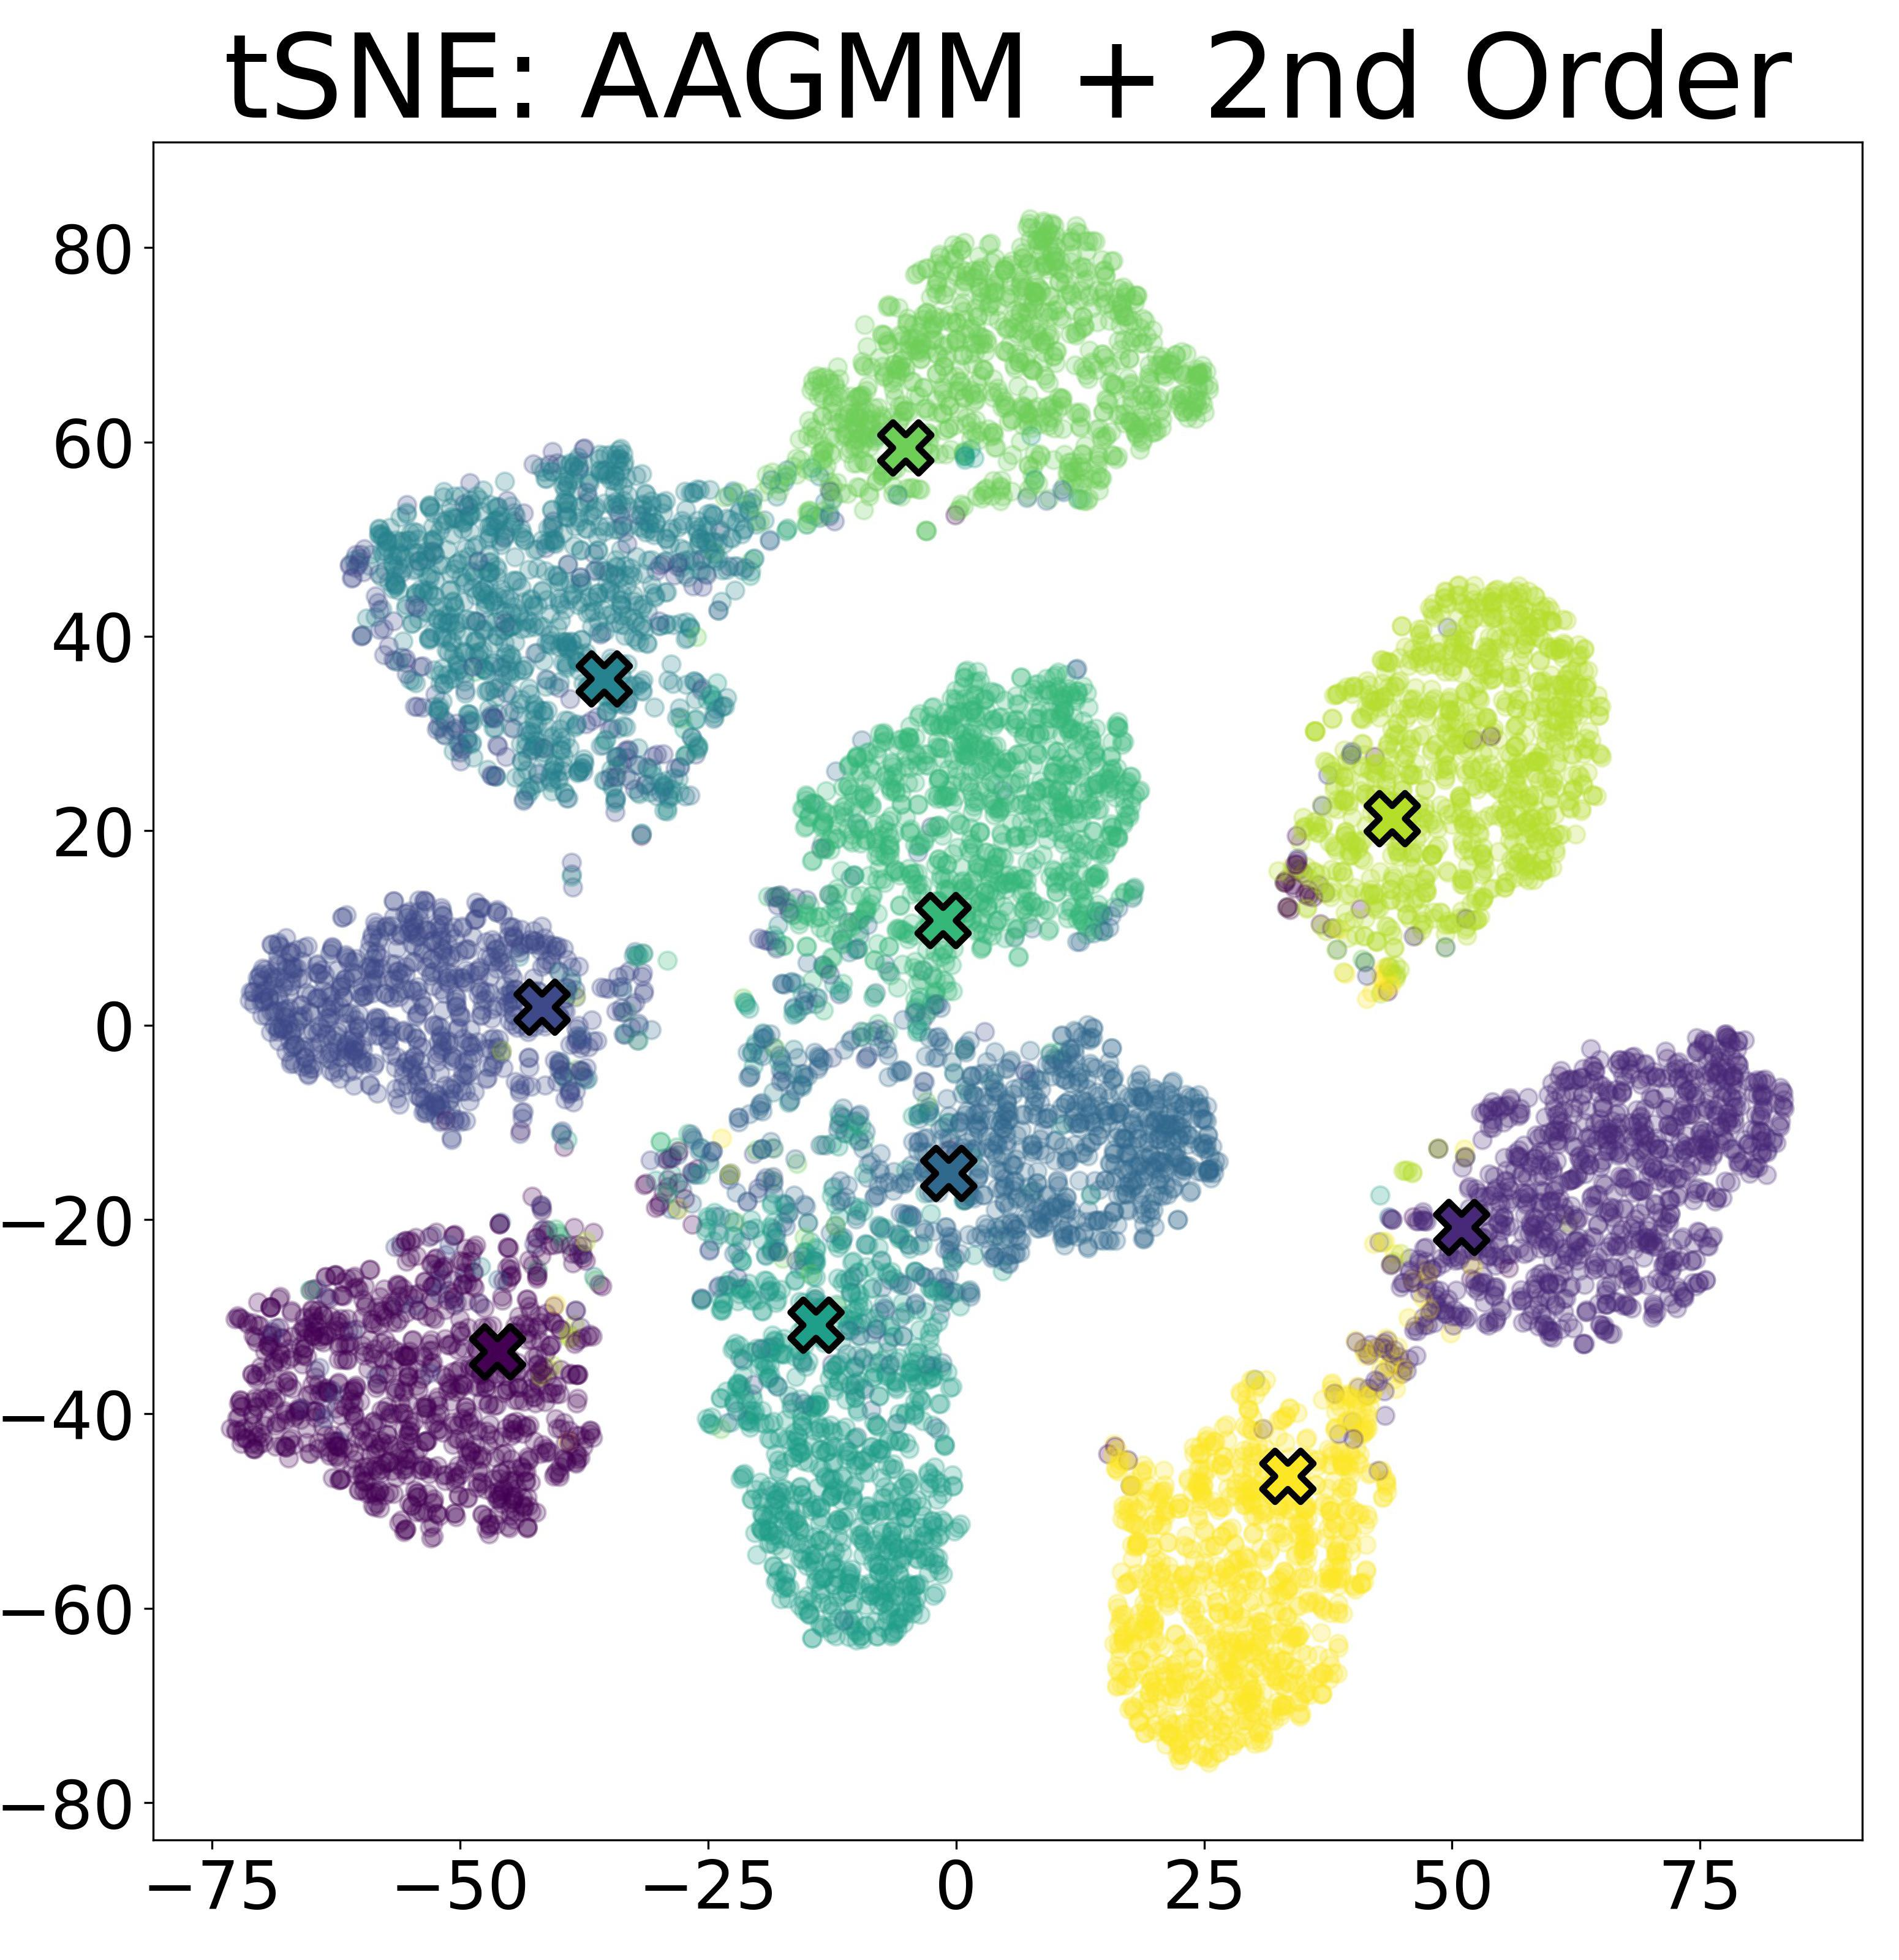
\includegraphics[width=.25\textwidth]{figures/id-00000054-tsne.jpg}}
	\subfloat{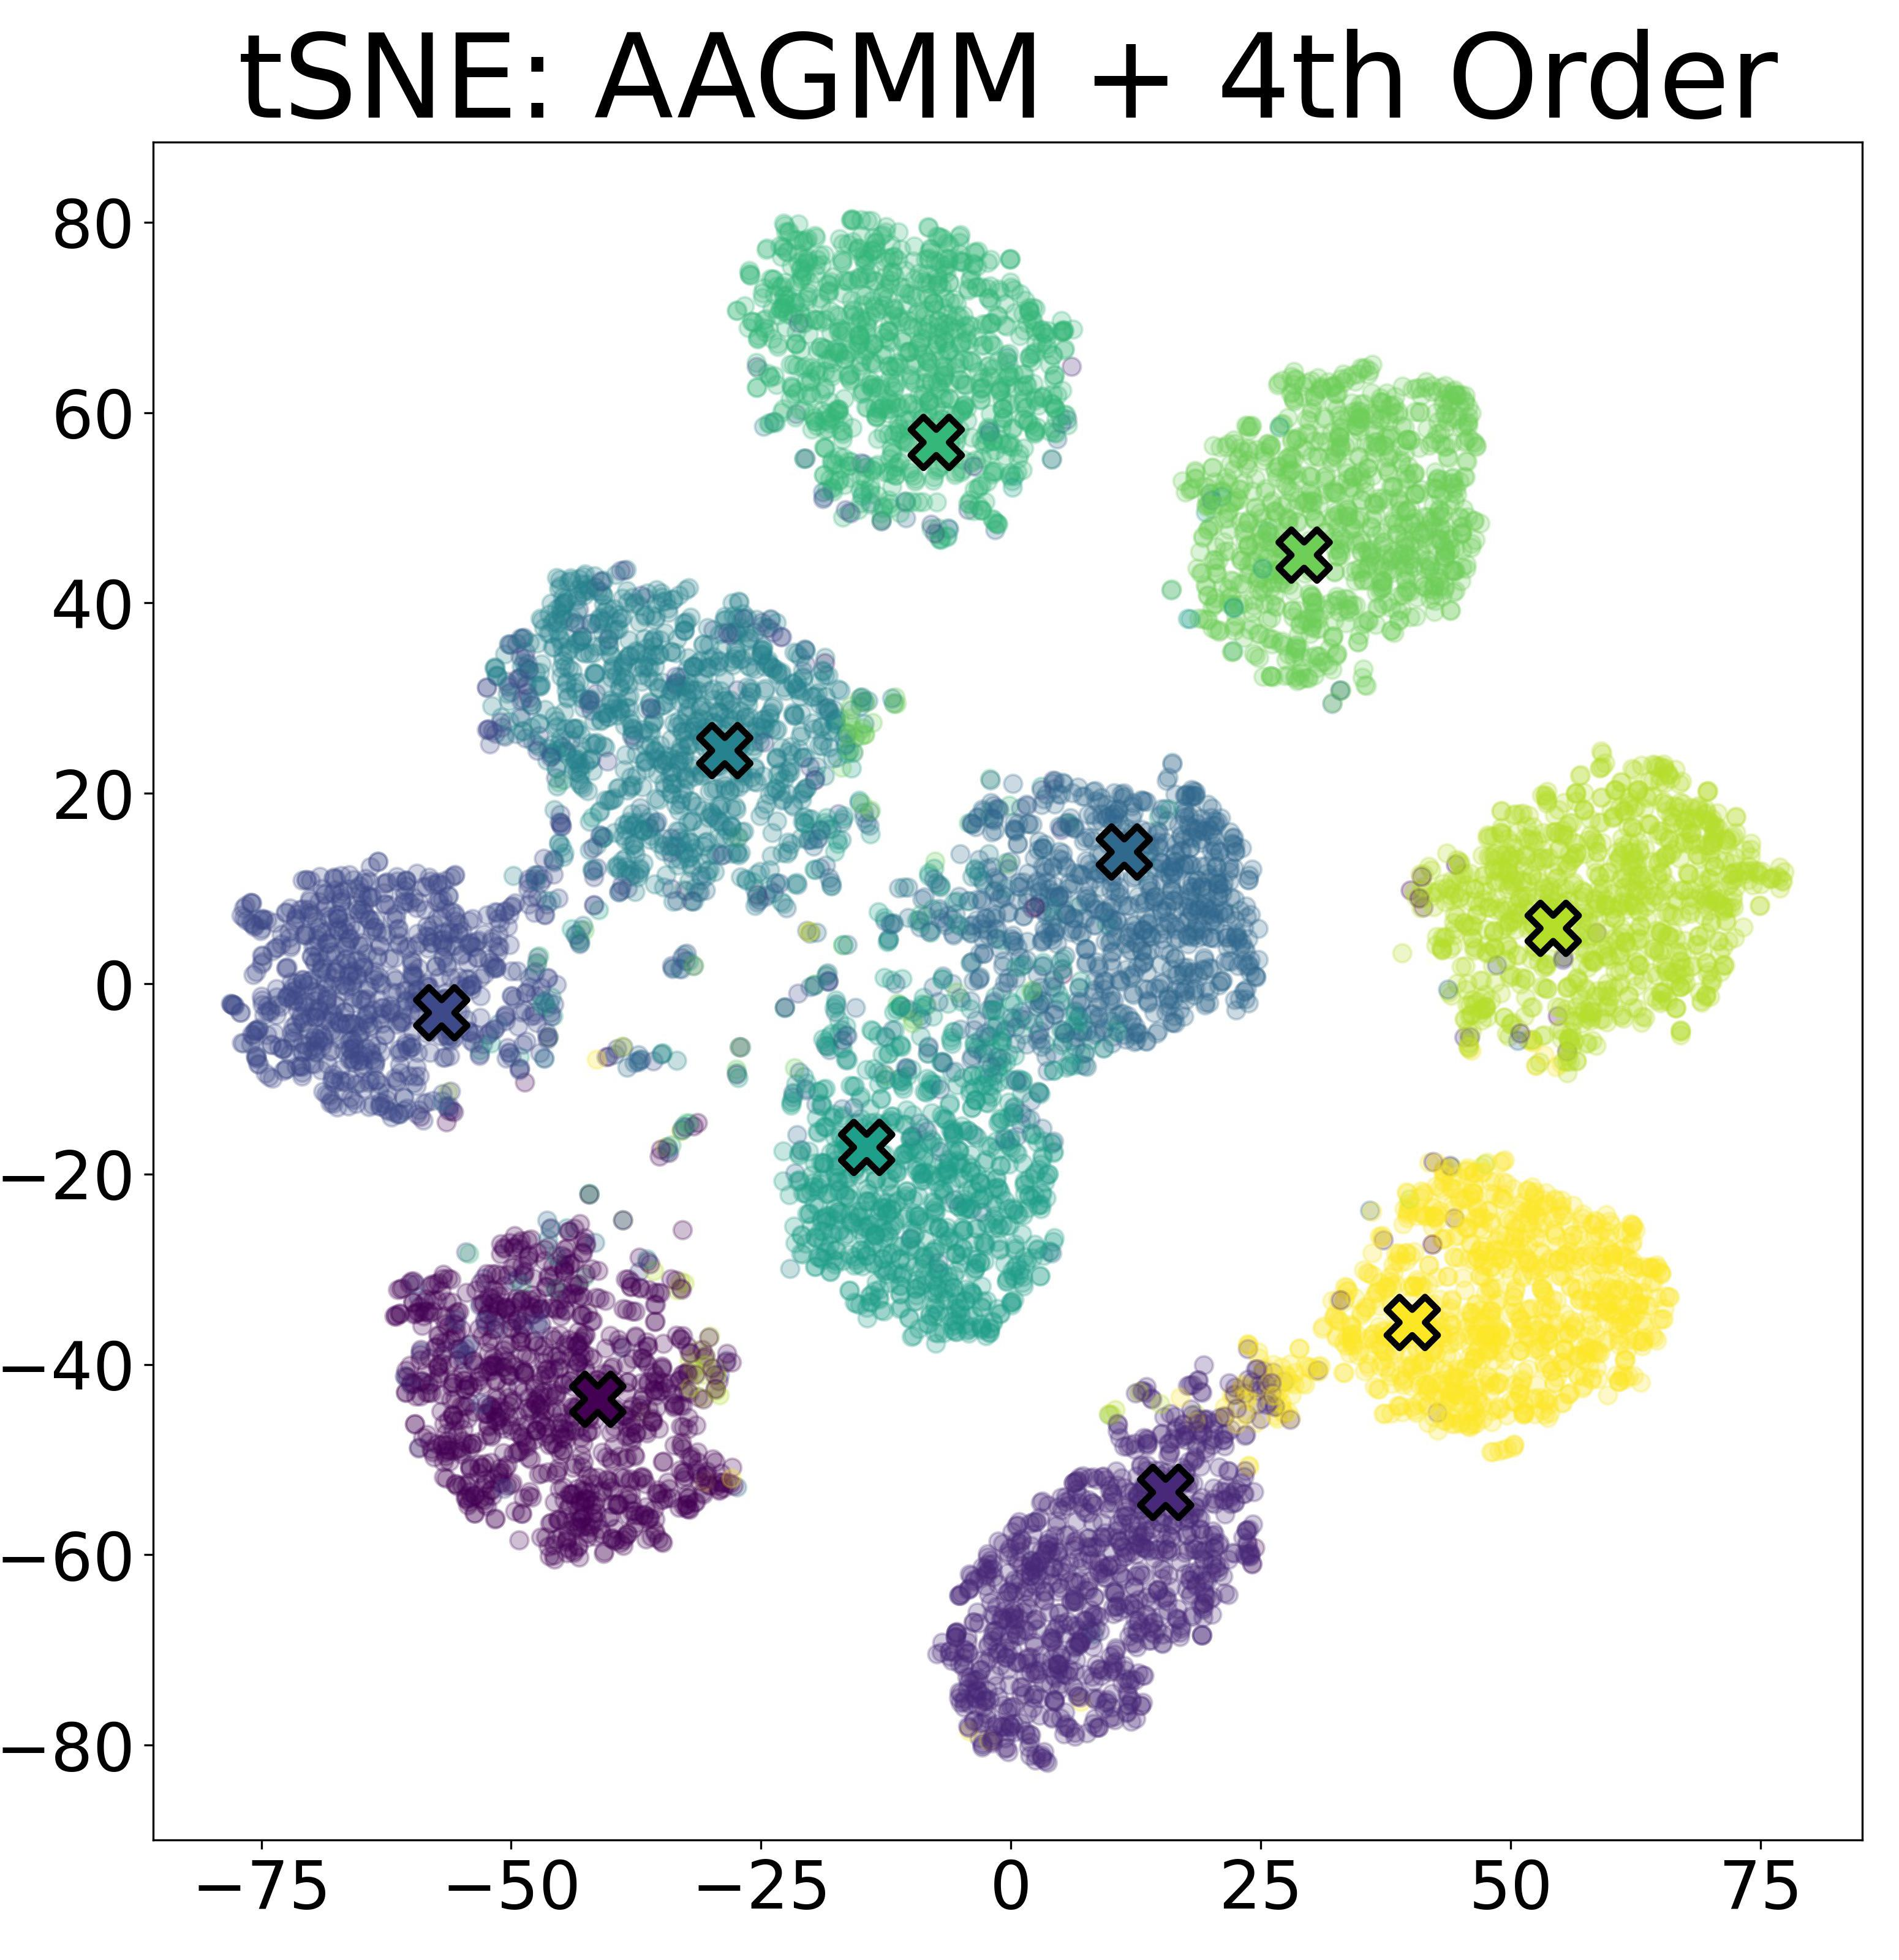
\includegraphics[width=.25\textwidth]{figures/id-00000021-tsne.jpg}}
	
	%	\includegraphics[width=0.9\linewidth]{example-image-a}
	\caption{t-SNE plot of the latent embedding space for various final layers with different MoM embedding constraints.} 
	\label{fig:cifar10tsne}
\end{figure*}

The majority of deep classifiers rely on a softmax final activation layer which predicts the conditional probability $p(y|x)$.
When that layer receives input $x$, the model predicts a soft psuedo-distribution of labels $y$ which argmax can convert into a hard label.
If $x$ is far from the decision boundary, then by definition, softmax assigns a prediction $y$ with high confidence.
This works well for inlier samples, well represented by the training distribution.
However, when presented with an outlier $x$, it is likely $x$ will be far from the decision boundary (\TODO{Figure ?}).
This means that softmax perceptrons, by definition, over-confidently hallucinate when given unexpected inputs \cite{wei2022mitigating}. 
Most deep classifiers use softmax without a safety net and thereby over-confidently predict $y$.
Ideally, when input $x$ is far from the decision boundary and training exemplars, the model should not be confident about the output class label $y$.

Replacing softmax with a generative method that models the joint probability $p(y,x)$ can improve the capability of deep classifiers. 
Models using a final layer capable of learning the joint probability $p(y,x)$ can infer the conditional $p(y|x)$.
More importantly, such a layer can also infer the prior probability $p(x)$.
Thus, if $x$ is an unexpected input, then such layer can flag the input as a low-probability outlier, rather than confidently predicting a label.

% TODO rewrite paragraph to remove weird conversational tone
Although there is related work in creating a generative final activation layer, there is an open question of how best to train such a layer in a deep learning context.  \TODO{(chapman) Citations for the related work...?}
The straw-man’s approach would be to minimize the cross entropy between $y$ and $y\_pred$ as usual.  
Figure \ref{fig:cifar10tsne} shows actual t-SNE plots for semi-supervised CIFAR-10 \cite{cifar10} classification that beautifully illustrate why such an approach will not work as intended.  
Figure \ref{fig:cifar10tsne} (top-right) shows the latent space of a classification model that is $93\%$ accurate on the test set, yet the cluster centers are not even remotely located anywhere nearby the data points at all.  
If one only cares about predictive performance, then one might conclude such a strange model would suffice.  
But if one needs a robust model, then simply fitting the decision boundary is not adequate, we need to learn the full latent distribution. 
Figure \ref{fig:cifar10tsne} (bot) shows that with our MoM embedding constraints, the exact same model can achieve comparable if not better accuracy, but with the added benefit of modeling the true location of cluster centers in the latent space.

%\begin{figure}[ht]
%	\centering
%	\subfloat{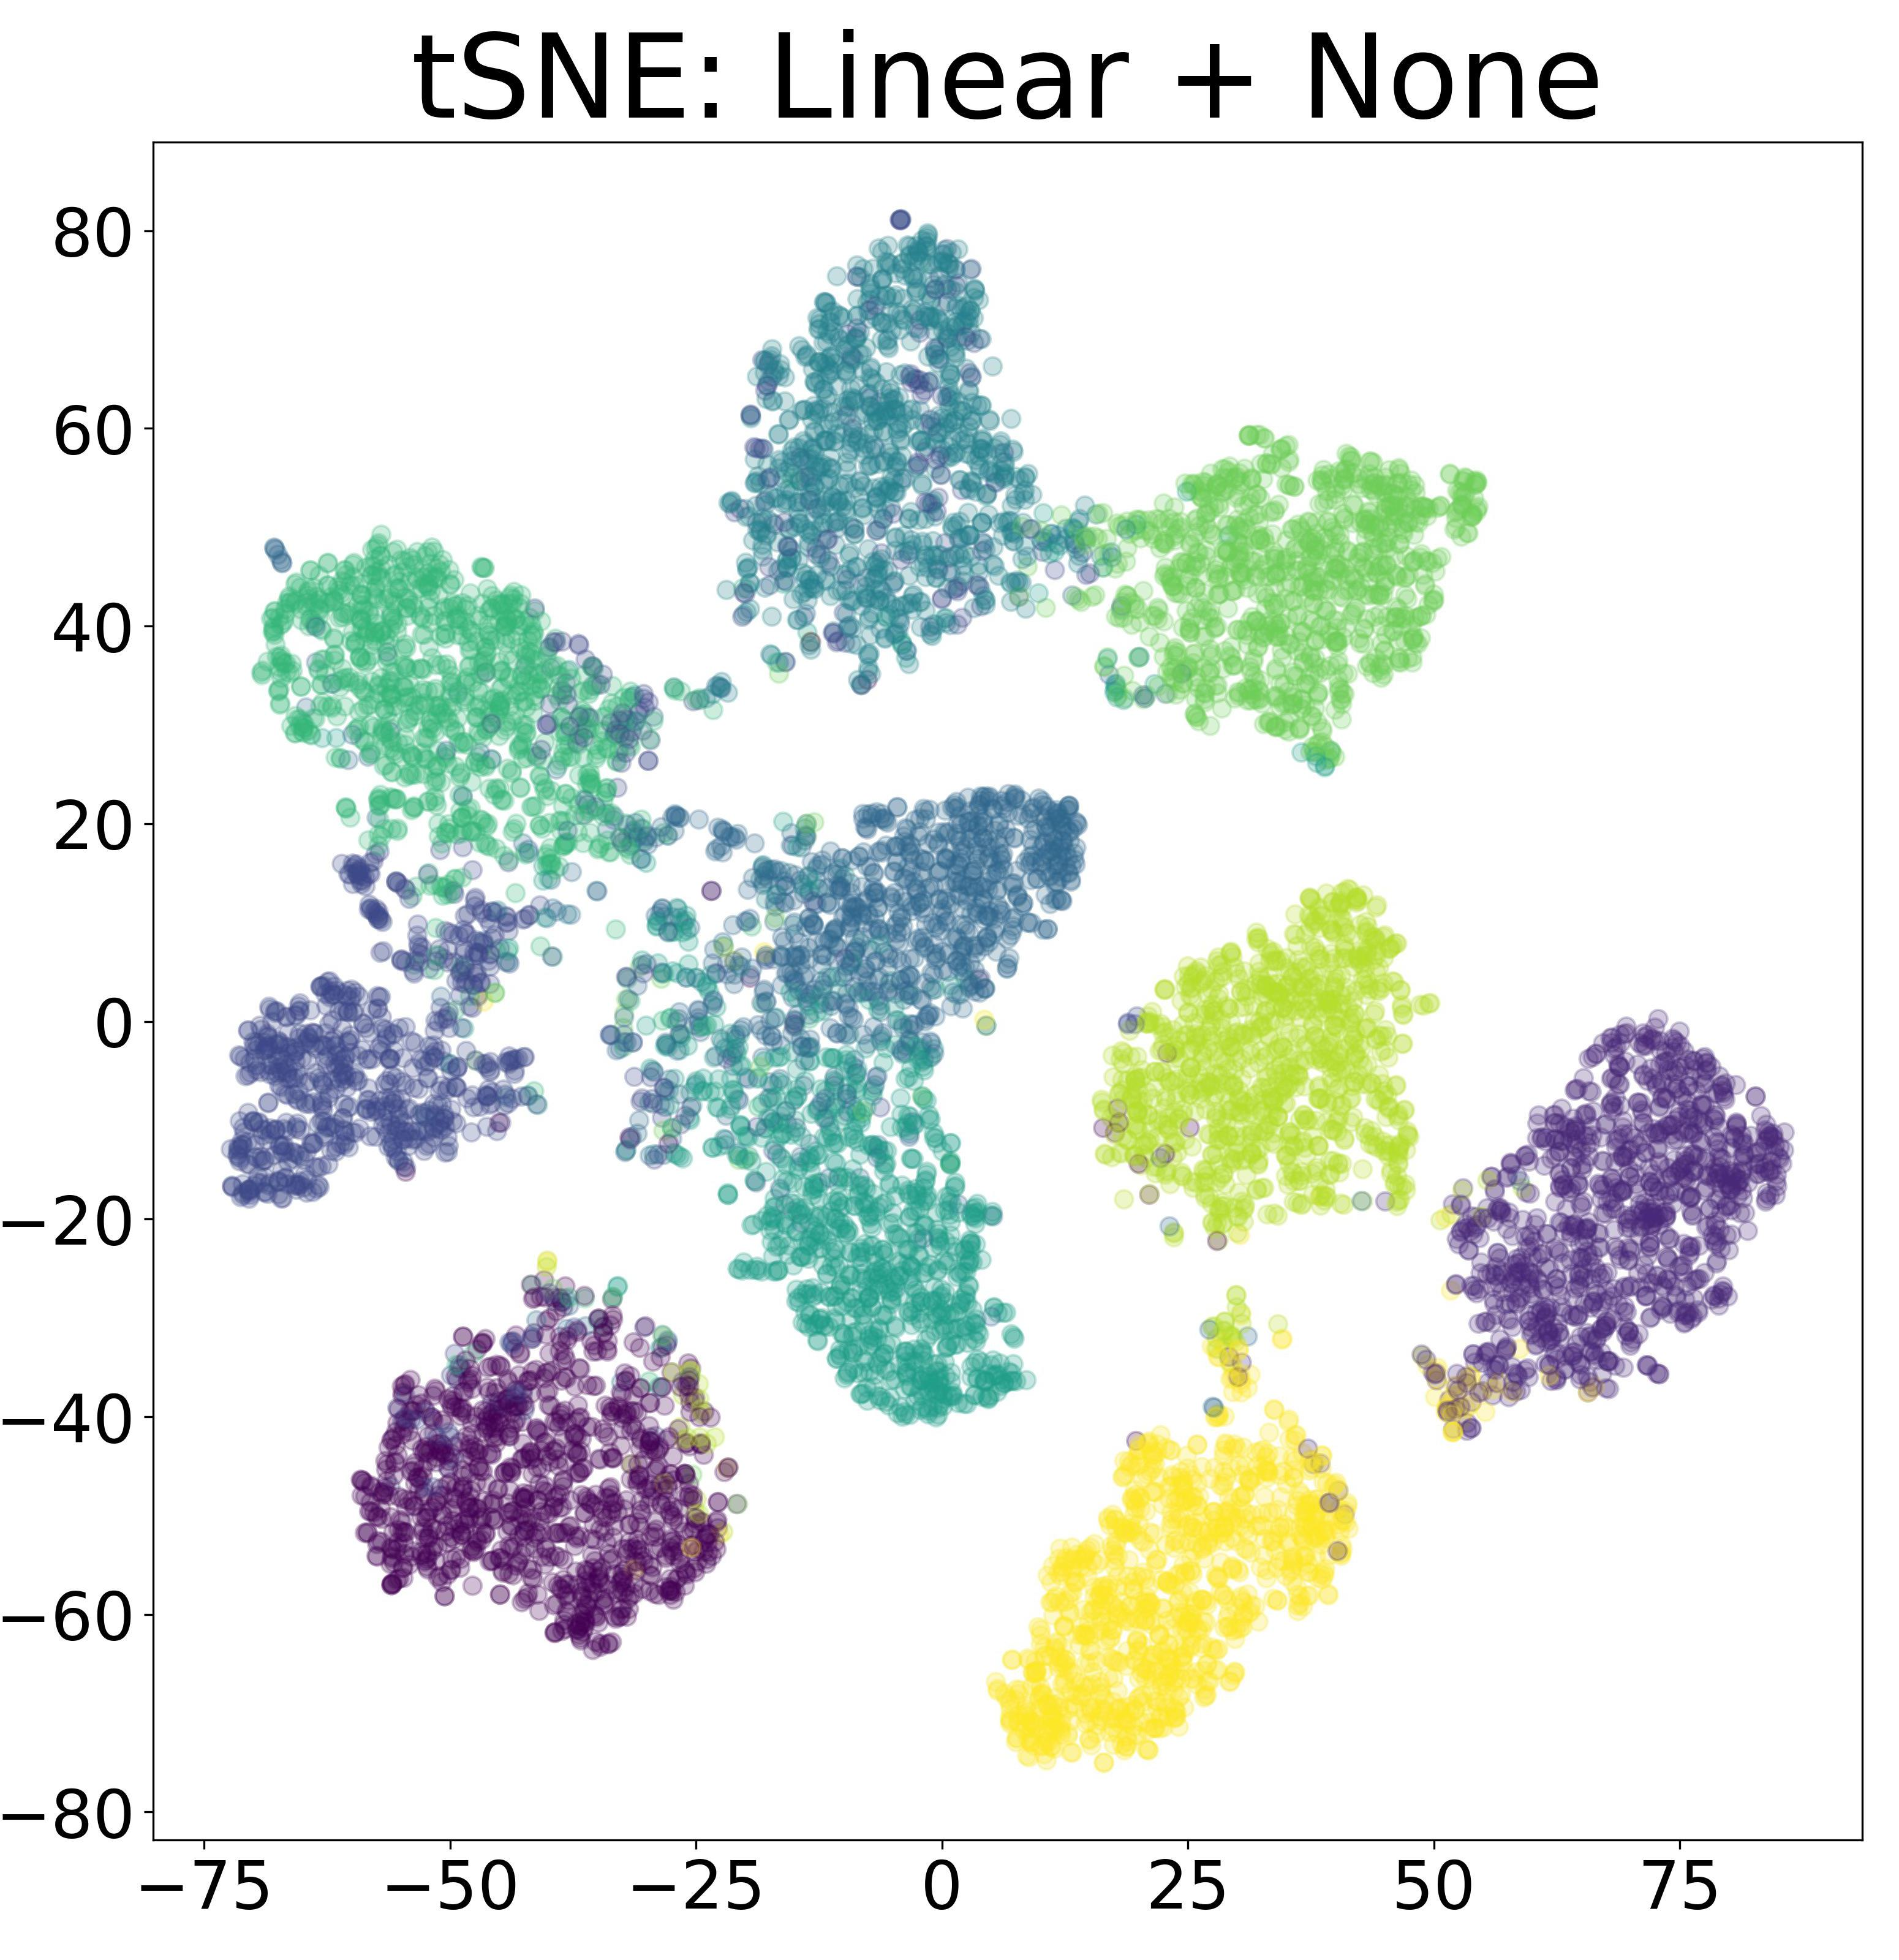
\includegraphics[width=.5\columnwidth]{figures/id-00000001-tsne.jpg}}
%	\subfloat{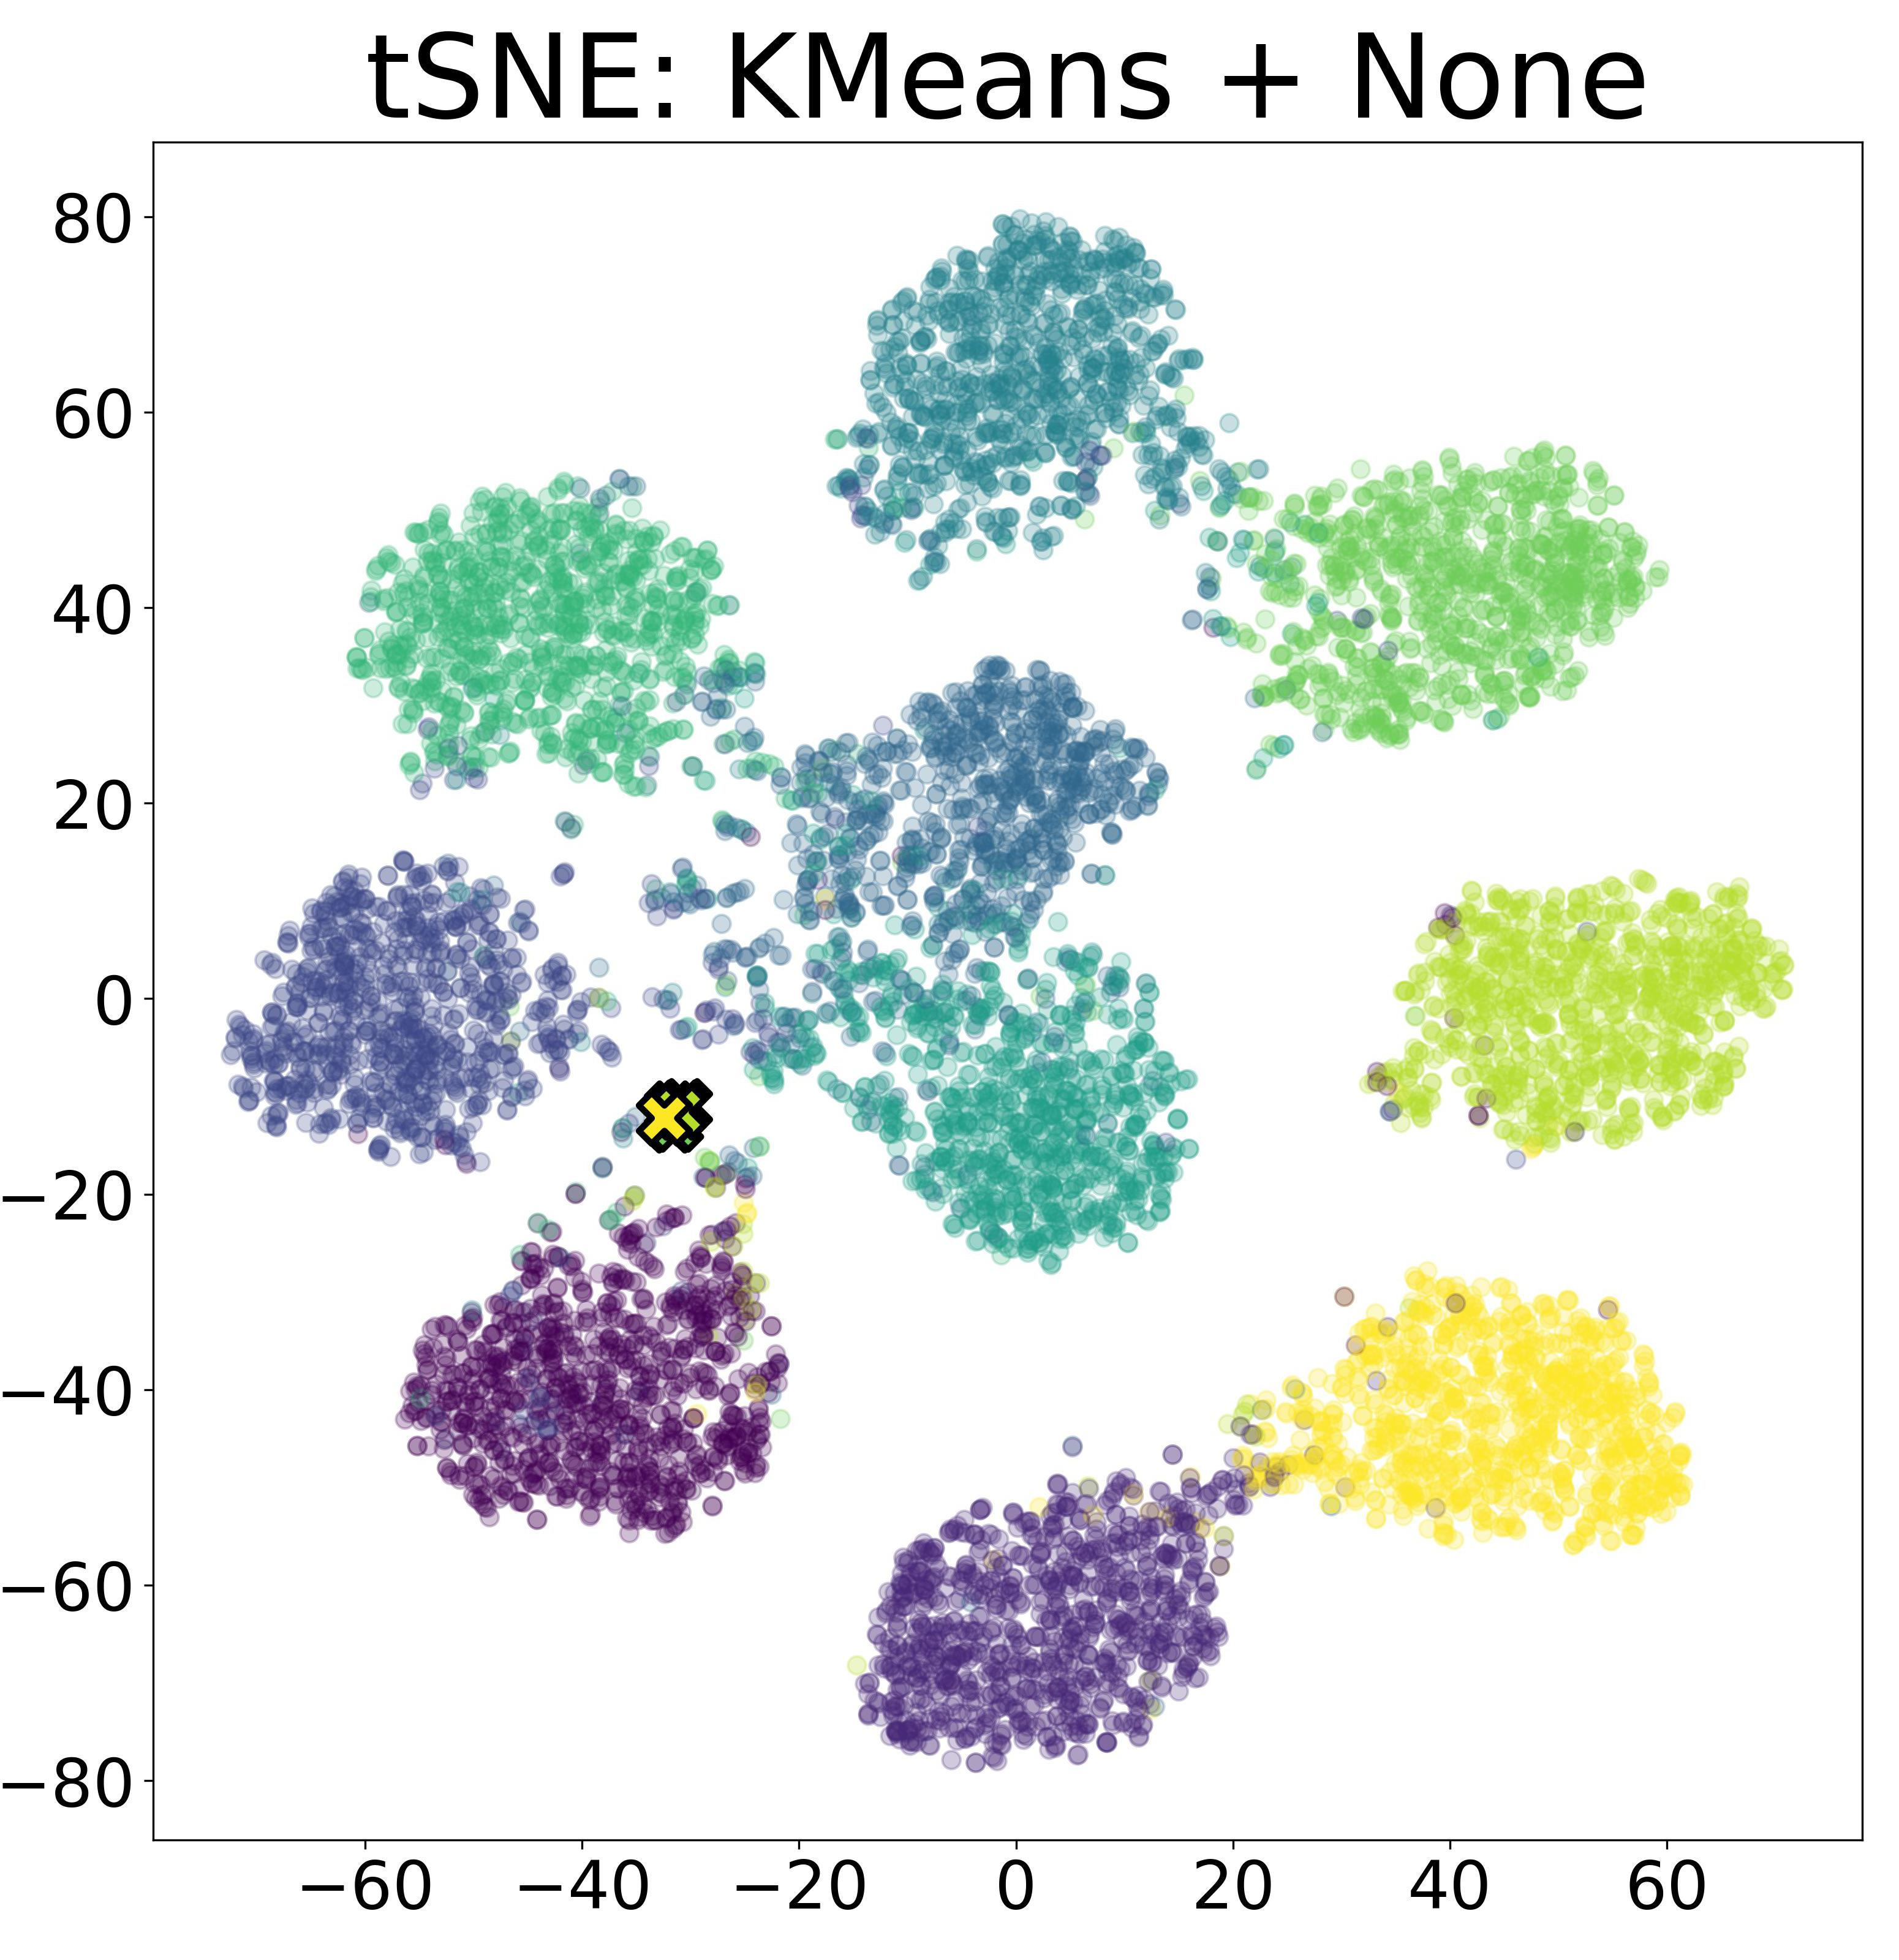
\includegraphics[width=.5\columnwidth]{figures/id-00000013-tsne.jpg}}
%	\\
%	\subfloat{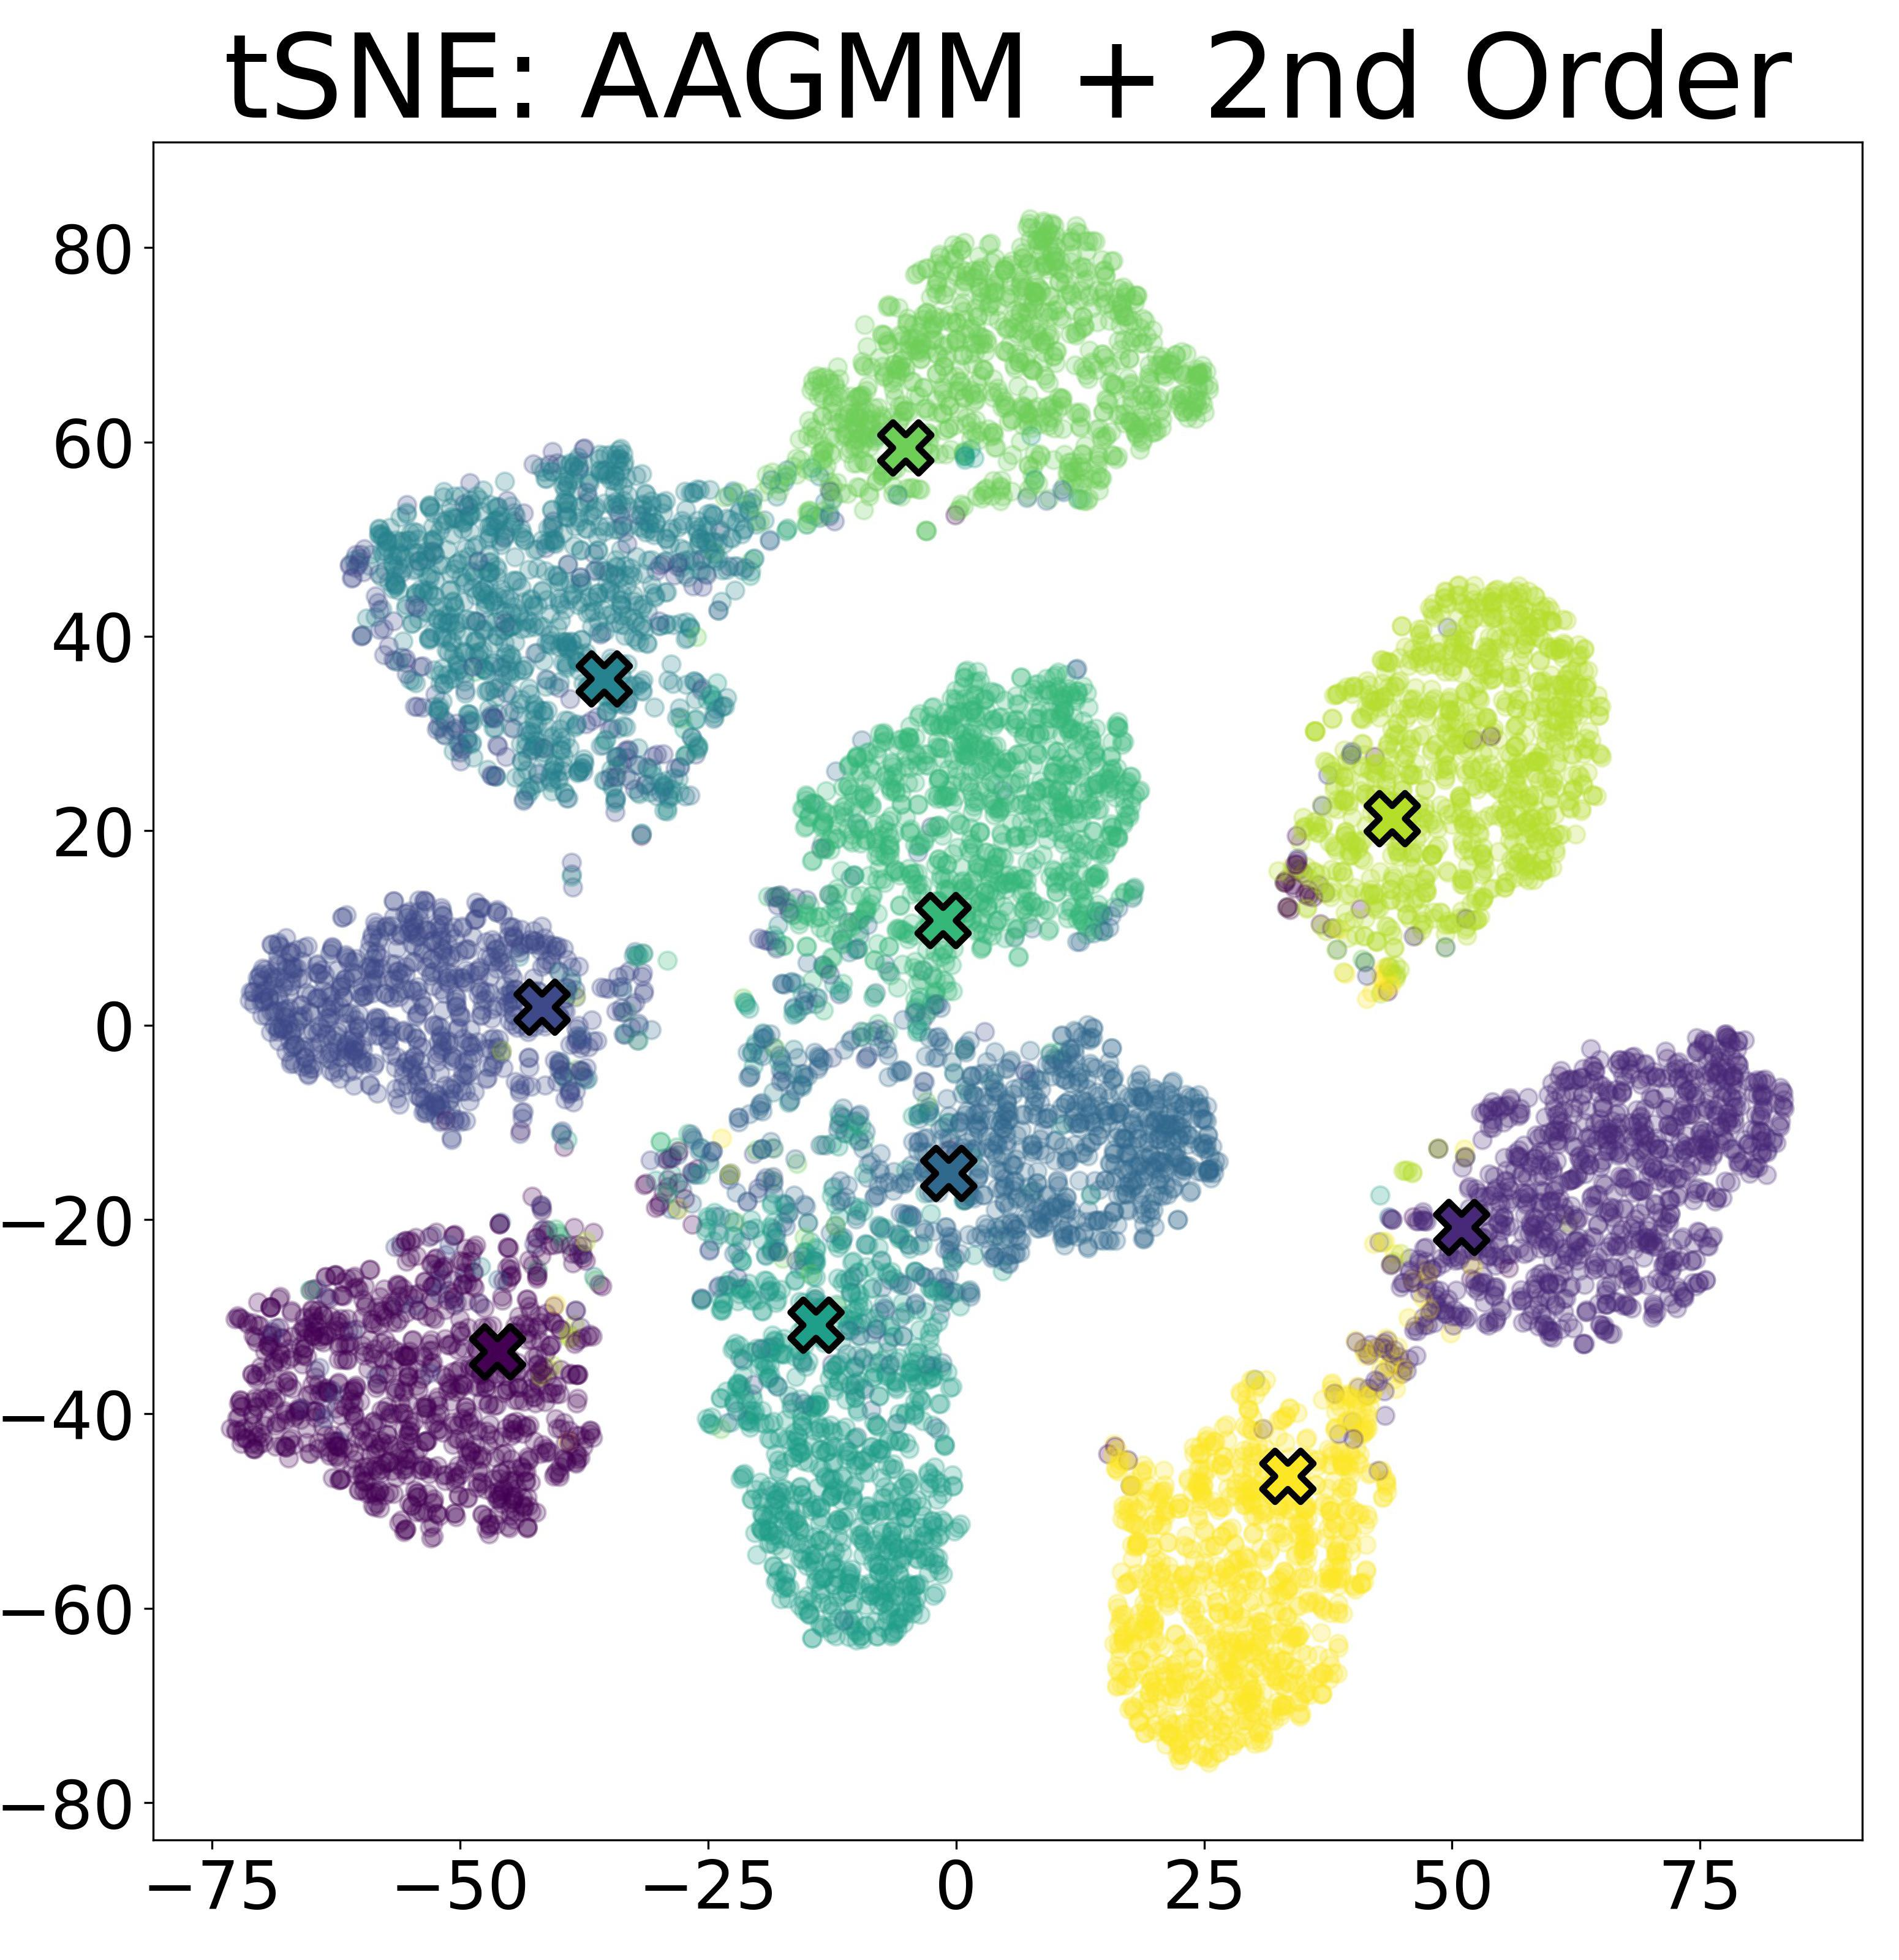
\includegraphics[width=.5\columnwidth]{figures/id-00000054-tsne.jpg}}
%	\subfloat{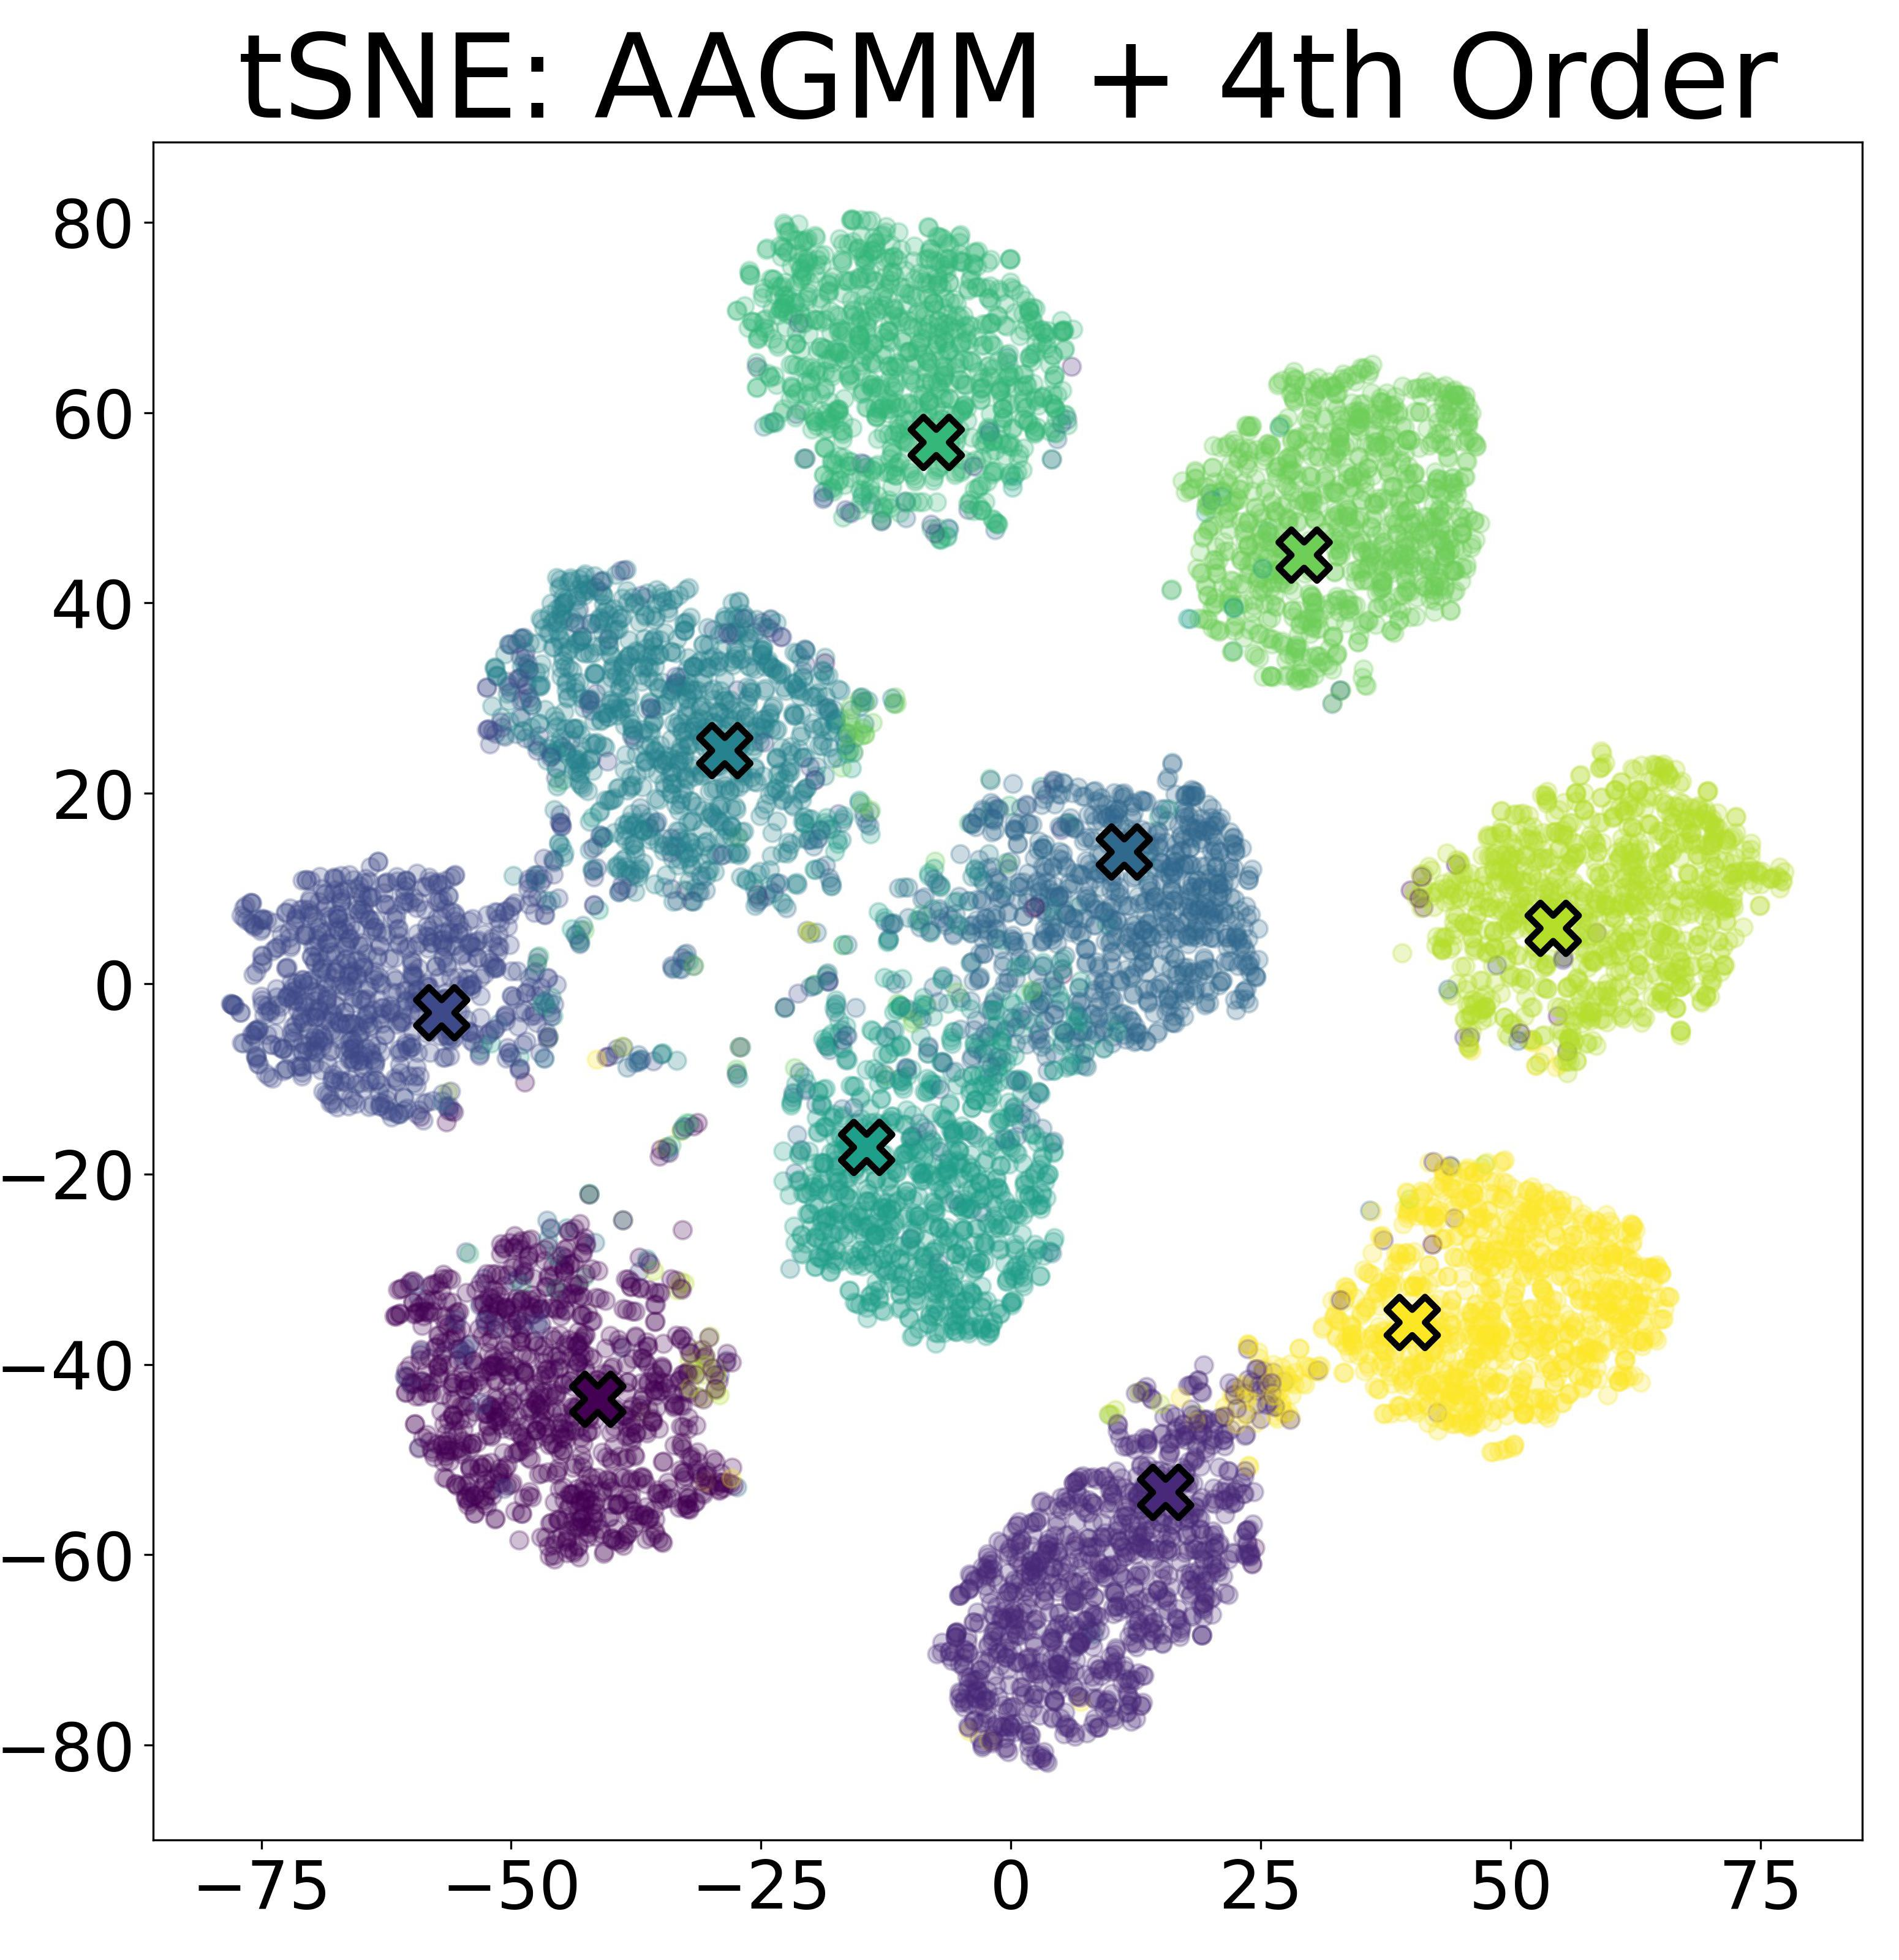
\includegraphics[width=.5\columnwidth]{figures/id-00000021-tsne.jpg}}
%	
%	%	\includegraphics[width=0.9\linewidth]{example-image-a}
%	\caption{t-SNE plot of the latent embedding space for various final layers with different MoM embedding constraints.} 
%	\label{fig:cifar10tsne}
%\end{figure}


This work argues that Semi-supervised learning (SSL) pseudo-labeling methods can be improved with better calibration of the network logits used to filter reliable pseudo-labels from the unreliable ones. 
This is equivalent to improving the accuracy of class inlier determination.
SSL is an excellent application to test generative final activation layers which model the join probability $p(y,x)$, as pseudo-labeling methods are sensitive to outliers.

SSL leverages an abundance of unlabeled data to improve deep learning based model performance under limited training data regimes \cite{zhu2022introduction,li2019safe,hady2013semi}.
%Image classification has become a playground for exploring novel SSL ideas, of which there are several flavors.
Contrastive learning methods leverage the intuition that similar instances should be close in the representation space, while different instances are farther apart \cite{yang2022class,li2021comatch}.
Consistency regularization borrows the intuition that modified views of the same instance should have similar representations and predictions \cite{sohn2020fixmatch,lee2022contrastive,zhang2021flexmatch,kim2022conmatch}.
Pseudo-labeling methods like FixMatch \cite{sohn2020fixmatch} leverage the ideas of consistency regularization.
This works contributes:

\begin{enumerate}
	\item A replacement of the final linear+softmax final activation layer of the neural network with either an axis-aligned differentiable Gaussian Mixture Model (AAGMM) or an equal variance version named KMeans trained via back prop, both of which have explicit modeling of class cluster centroids. 
	\item A demonstration on the latent embedding space reacts to various constraints on how it should be structured by adding penalties if the per-class clustering does not conform to between 0 and 4 of the first gaussian moments being identity/zero \cite{pearson1936method}.
\end{enumerate}

%This paper explores the impacts of replacing the final linear layer of a network with a generative model and embedding space constraints.
%This combination demonstrates improvements in final model accuracy when using pseudo-labeling methods where very few annotations are available.
We demonstrate this methodology using the standard CIFAR-10 benchmark dataset with 40 and 250 labels\cite{cifar10}. %) and CIFAR-100 (400 and 2500 label) benchmarks \cite{cifar10}. 
%Additionally, we explore the impact high level prescriptive constraints on the embedding space have on the resulting trained model. 
Finally, because the embedding constraint penalties are applied to all unlabeled data and not just the valid pseudo-labels, our method extracts training signal from every unlabeled data point, an improvement on baseline pseudo-labeling methods (like FixMatch \cite{sohn2020fixmatch}) which only learn from the valid pseudo-labels.


\section{Related Work}

% TODO compare our method to lee2022contrastive which uses explicit cluster centers, and draws both the valid and non valid PL to the cluster center, just like we do, we just don't have a contrastive element like they do

Semi-Supervised learning has shown great progress in learning high quality models, in some cases matching fully supervised performance for a number of benchmarks \cite{zhang2021flexmatch}.
The goal of SSL is to produce a trained model of equivalent accuracy to fully supervised training, with vastly reduced data annotation requirements.
Doing so relies on accurately characterizing inlier vs outlier unlabeled samples.

\subsection{Pseudo-Labeling}
Self-supervised learning was among the initial approaches employed in the context of semi-supervised learning to annotate unlabeled images. 
This technique involves the initial training of a classifier with a limited set of labeled samples and incorporates pseudo-labels into the gradient descent process, exceeding a predefined threshold \cite{yarowsky1995unsupervised, mcclosky2006reranking, olivier2006semi,zhai2019s4l,livieris2019predicting,rosenberg2005semi,menon2020deep}. 
A closely related method to self-training is co-training, where a given dataset is represented as two distinct feature sets \cite{blum1998combining}. 
These independent sample sets are subsequently trained separately using two distinct models, and the sample predictions surpassing predetermined thresholds are utilized in the final model training process \cite{blum1998combining,prakash2014survey}.
A notably advanced approach to pseudo-labeling is the Mean Teacher algorithm \cite{tarvainen2017mean}, which leverages exponential moving averages of model parameters to acquire a notably more stable target prediction. 
This refinement has a substantial impact on enhancing the convergence of the algorithm.


\subsection{Consistency Regularization}

Consistency regularization operates on the premise that when augmenting an unlabeled sample, its label should remain consistent. 
This approach implicitly enforces a smoothness assumption, promoting coherence between unlabeled samples and their basic augmentations \cite{xie2020unsupervised}. 
In other words, the model should be able to predict the unlabeled sample $x$ exactly the same way it predicts the class for $Augmented(x)$ \cite{berthelot2019mixmatch,sohn2020fixmatch,berthelot2019remixmatch,mustafa2020transformation}. 
In addition to evaluating image-wise augmentations, recent research has demonstrated that incorporating class-wise and instance-based consistencies yields superior performance outcomes \cite{zheng2022simmatch,li2021comatch}. 
Similarly, using consistencies between the predictions and low-dimensional embeddings from the unlabeled image strong and weak augmentations in a graph based setup demonstrates improvement over class-wise and instance-based consistencies \cite{zheng2023simmatchv2}.
Finally, pseudo-labeling filtering based on consistence between strongly augmented views, gaussian filtering and embedding based nearest neighbor filtering shows convergence improvement \cite{kim2022conmatch,menon2022semisupervised}.

\subsection{Latent Embedding Constraints}

Several papers have attempted to enhance the quality of pseudo-labels to either improve the final model accuracy, improve the rate of convergence, or avoid confirmation bias \cite{arazo2020pseudo}.
Rizve et al. \cite{rizve2021defense} explores how uncertainty aware pseudo-label selection/filtering can be used to reduce the label noise.
Incorrect pseudo-labels can be viewed as a network calibration issue \cite{rizve2021defense} where better network logit calibration might improve results \cite{Xing2020DistanceBased}.
Improvements to the pseudo-labeling process have been demonstrated by imposing curriculum \cite{zhang2021flexmatch} or by including a class-aware contrastive term \cite{yang2022class}.
Leveraging the concept of explicit class cluster centers for conditioning semantic similarity improves final model accuracy \cite{zheng2022simmatch}.
Additionally, improvements have been found in extended purely clustering based methods like DINO \cite{caron2021emerging} into semi-supervised methods \cite{fini2023semi}.

% TODO talk about SimMatch embedding constraint via semantic seimilarity?

\section{Methodology}

In this section, we explore our proposed replacement final activation layers and our embedding space constraints.
FixMatch \cite{sohn2020fixmatch} is a simple, well performing SSL algorithm.
As such, it serves as a good comparison point for exploring the effect of our contributions.
Our methodology is based upon the published FixMatch \cite{sohn2020fixmatch} algorithm, with identical hyper-parameters unless otherwise stated.
We extend FixMatch with a few minor training algorithm modifications explored in the Hyperparameters Section \ref{hyperparams}.

Both the linear layer replacements and the embedding constraints explored herein represent increasing levels of prescription about how the final latent embedding space should be arranged compared to a traditional linear layer.
The idea of leveraging clusters in embedding space is not new \cite{caron2018deep,caron2020unsupervised,enguehard2019semi}, but we extend the core idea with a novel differentiable model with learned cluster centroids and MoM based constraints.

\subsection{Alternate Final Layers}

A limitation of traditional final activation layers such as linear+softmax is that they are fully discriminative; i.e. they estimate the posterior $p(Y|X)$, but do not attempt to model the sample distribution $p(X)$ or the joint probabilities $p(Y,X)$. 
To overcome this limitation, we present two semi-parametric final activation layers (a) the Axis Aligned GMM (AAGMM) layer, and (b) an equal variance version of AAGMM that we henceforth call the KMeans activation layer due to the similarity of the objective function with a gradient based KMeans.

These activation layers are fully differentiable and integrated into the neural network architecture as a module in the same way as a traditional final linear layer. 
As such, they do not require external training and do not use expectation maximization.
They are drop in replacements for the final linear layer.

Importantly, these activation layers exhibit both discriminative and generative properties. 
The neural network model $F(X;\theta_F)$ transforms the data $X$ into a latent space $Z = F(X;\theta_F)$, and the final activation layer estimates the probability densities $p(X)$, $p(Y;X)$ and $p(Y|X)$ by fitting a parametric model to the latent representation $Z$.

\subsubsection{Axis Aligned Gaussian Mixture Model Layer}

The AAGMM layer defines a set of $K$ trainable clusters, one cluster per label category. 
Each cluster $k=1 \dots K$ has a cluster center $\mu_k$ and cluster covariance $\Sigma_k$. 
The prior probability of any given sample $X_i$ is defined by the mixture of cluster probability densities over the latent representation $Z_i$ as follows,

\begin{equation}
	\begin{aligned}
		\label{eq_px}
		&p(X_i) = \sum_{k=1}^K \mathcal{N} (Z_i, \mu_{k}, \Sigma_k)
		\\[10pt]
		&\textit{where} \quad Z_i = F(X_i, \theta_F)
	\end{aligned}
\end{equation}

Where $\mathcal{N}(Z_i, \mu_k, \Sigma_k)$ represents the multivariate gaussian pdf with centroid $\mu_k$ and covariance $\Sigma_k$. 
AAGMM is axis aligned because $\Sigma_k$ is a diagonal matrix, as such the axis-aligned multivariate normal pdf simplifies to the marginal product of Gaussians along each of the $D$ axes as follows,

\begin{equation}
	\begin{aligned}
		\mathcal{N} (X_i, \mu_{k}, \Sigma_k) &=  \prod_{d=1}^D \frac{1}{\sigma_{k,d}\sqrt{2 \pi}} exp \Big( \frac{Z_{i,d} - \mu_{k,d}} {\sigma_{k,d}} \Big)^2 \\[10pt]
		&\textit{where} \quad \sigma^2_{k,d} = \Sigma_{k,d,d}
	\end{aligned}
\end{equation}

As there is one cluster per label category, the joint probability for sample $i$ with label assignment $k$, $p(Y_{i,k},X_i)$ is the given by the normal pdf of the $k^{th}$ cluster,

\begin{equation}
	\label{eq_pyx}
	p(Y_{i,k},X_i) = \mathcal{N} (Z_i, \mu_{k}, \Sigma_k) \end{equation}

By Bayesian identity, the posterior probability $\hat{Y}_k=p(Y_{k}|X_i)$ can therefore be inferred from eq \ref{eq_px} and \ref{eq_pyx} as follows,

\begin{equation}
	\hat{Y}_{i,k} = p(Y_{i,k}|X_i) = \frac{p(Y_{i,k}, X_i)}{p(X_i)}
\end{equation}

The AAGMM layer is implemented as a normal PyTorch \cite{pytorch} module.
It has two parameters updated by backprop.
(1) the explicit cluster centers, a matrix $num\_classes \times embedding\_dim$ initialized randomly, and
(2) the diagonal elements of the $Sigma$ matrix, randomly initialized in the range $[0.9, 1.1]$, which contains the diagonal elements of the GMM Sigma matrix for each cluster.

\subsubsection{KMeans Layer}

We also implement a KMeans final layer which is a more restrictive form of the AAGMM layer.
The KMeans layer is additionally constrained such that the gaussian covariance matrix $\Sigma_k$ for each cluster center $k$ is the $[D \times D]$ identity matrix. 
This constraint yields spherical cluster centers; similar to how the traditional KMeans algorithm also assumes spherical clusters.
%It is notable, that in both cases, the AAGMM layer and the KMeans layer are not trained using the KMeans algorithm, or with any form of expectation maximization.  Rather, they are trained by gradient descent as a fully integrated module within the network architecture.  

%The KMeans activation layer defines a set of C trainable cluster centers, one cluster center per label category.  This layer is called a KMeans layer because, like KMeans, it makes use of equal-variance gaussians to define the prior $p(X)$.  However, it is not trained using the KMeans algorithm, but instead by making use of cross entropy loss as part of the neural network model.  We define $K$ $D$-dimensional cluster centers $\mu_1 \ldots \mu_K$, one center per label category.  This constitutes a generative model, where the prior probability of any given sample $X_i$ is defined in terms of the cluster centers as follows

The KMeans layer is also implemented as a normal PyTorch \cite{pytorch} module.
The explicit cluster centers is a learned parameter updated by backprop.
See the published codebase for implementation details about the AAGMM and KMeans layers.




\subsection{Method of Moments Embedding Constraints}

We introduce and evaluate a series of embedding constraints based on the Method of Moments (MoM) \cite{pearson1936method} in order to fit the semi-parametric latent prior parameters.  
The latent prior $p(X_i)$ is calculated in equation \ref{eq_px} and then used to infer the posterior $p(Y_{i,k}|X_i)$.
As usual, the posterior is trained using cross entropy loss.  
When embedding constraints are omitted, it is possible for the model to learn an accurate decision boundary for the posterior without modeling the latent prior.

Our novel last layer is semi-parametric, because the prior is a parametric model of the latent distribution $Z$ which is the result of a neural network feature extraction $F(X;\theta)$. 
Therefore, attempting to fit the GMM directly to $Z$ using Maximum Likelihood (ML) or simple Expectation Maximization (EM), is not appropriate, because doing so would fail to learn an appropriate feature space for discrimination.
MoM solves these problems and is an appropriate strategy for semi-parametric models including ours.

The MoM relies on the use of \textit{consistent estimators}, which asymptotically share sample and population statistics.
Assume that $z$ is a finite sample of $n$ elements drawn from infinite population $Z$, then a series of $P$ well-behaved sample statistics $g_p$ should very closely approximate their $k$ population statistic as follows,

\begin{equation}
	\forall p=1 \dots P \quad
	\frac{1}{n} \sum_{i=1}^n g_p(z_i) \approx E(g_p(Z))
\end{equation}

We can therefore constrain the latent representation of our model to approximate an independent joint Gaussian distribution. 
In the univariate gaussian case, the $p^{th}$ order centralized moment constraint is the following.

\begin{equation}
	E\left[ (Z-\mu)^p \right] = 
	\begin{cases} 
		0 &  \text{if} \; p \; \text{is odd} \\
		\sigma^p(p - 1)!! & \text{if} \; p \; \text{is even}
	\end{cases}
\end{equation}

By this formula, the univariate unit gaussian has mean $0$, standard deviation $1$, skew $0$, and kurtosis $3$.

In the joint multivariate case, each dimension is independent by definition.  As such, if we redefine $Z$, $\mu$, and $p$ to be all $D$ dimensional, then the centralized joint gaussian moment can be defined as follows,

\begin{equation}
	E\left[g_p(Z - \mu)\right] = E\left[ \prod_{d=1}^D (Z_d - \mu_d)^p_d \right]
\end{equation}

Due to independence of the axes, this moment can be represented as a product of univariate moments of the individual gaussians as follows,

\begin{equation}
	E\left[ \prod_{d=1}^D (Z_d - \mu_d)^p_d \right] = \prod_{d=1}^D E\left[ (Z_d - \mu_d)^p_d \right]
\end{equation}

The error (loss) term associated with the embedding constraint for any moment $p$ is equal to the L2 difference between the sample and population statistics as follows,

\begin{equation}
	\varepsilon_p = \left( \frac{1}{n} \sum_{i=1}^n g_p(z_i) - E(g_p(Z)) \right)^2
\end{equation}

Some moments are more important than others, and must be weighted more heavily.  
First order moments are simply the sample mean, and should be given the greatest weight as an embedding constraint.  
The second order moments form a sample covariance matrix, which ideally should be equal to the identity matrix, but the diagonal terms should be given greater weight than the off-diagonal terms.  
This is because, in a $D \times D$ covariance matrix, there are $D(D-1)$ off diagonal terms, but only $D$, diagonal terms.  
The $p^{th}$ order sample moments form a $p-1$ dimensional hyper-covariance matrix, with terms residing on the intersection of anywhere between $0$ and $p-1$ hyper-diagonals.  
To prevent over-representation of off-diagonal terms and encourage representation of on-diagonal terms, the loss function we use for any given moment term is inversely proportional to the number moment terms that share the same number of hyper-diagonals.  
This heuristic weighting scheme ensures that the overall contribution of each moment order is not overly influenced by the off-diagonal terms, and that the error weighting is therefore diagonally dominant.

\section{Experiments}

We evaluate both AAGMM and KMeans linear layer replacements and the embedding space constraints using our modified FixMatch\cite{sohn2020fixmatch} on the common SSL benchmarks CIFAR-10 \cite{cifar10} at 40 and 250 labels (4 and 25 labels per class). 
%When comparing against other SSL benchmark results (like SimMatch \cite{zheng2022simmatch}) it is unclear how the labeled samples were selected from the fully labeled dataset. 
We randomly selected 5 seed a priori for evaluation.
For each algorithm configuration tested one model was trained per seed.
During each run, the required number of labeled samples are drawn without replacement from the training population of the dataset in a deterministic manner (reproducible with the same seed).
All data not in this labeled subset is used as unlabeled data (i.e. the labels are discarded).


\begin{table}[h!]
	\begin{tabular}{r|c|c|c|c|c}
		\multicolumn{6}{c}{AAGMM+None on CIFAR-10 at 40 Labels}\\
		\hline
		Run Number & 1 & 2 & 3 & 4 & 5 \\
		\hline
		Test Accuracy \% & $94.6$ & $92.8$ & $92.8$ & $89.9$ & $86.4$ \\
	\end{tabular}
	\caption{Test accuracy for showing the run-to-run variance depending on the quality of the 40 labels selected from the full population.}
	\label{tab:runvariability}
\end{table}

As prior work \cite{sohn2020fixmatch} has noted, the resulting model quality is highly variable when only 4 samples are selected per class, as the quality and usefulness of the specific 4 samples can vary drastically. 
Table \ref{tab:runvariability} shows final test accuracy for the 5 AAGMM model runs with no embedding constraints, with the accuracy varying from $86\%$ to $94\%$.
Due to the potential for significant variance in the final model test accuracy, it can be informative to compare mean performance with max performance over the $N=5$ runs.
This explores both how well a method can be expected to do on average with random label sampling, vs how well it can potentially do with a more representative subset of labeled data.

\subsection{Hyper-Parameters}
\label{hyperparams}
% TODO reduce the WE in this section

\begin{table*}[ht!]
	\begin{tabularx}{\textwidth}{c|c|XXXXXX}
		\multicolumn{6}{c}{CIFAR-10 Mean Test Accuracy} \\ \hline\hline
		Last Layer &   Emb Dim   & \multicolumn{5}{c}{40 Labels (5 trials)}            \\ 
		\hline
		Embedding Constraint  &  & None & $1st$ Order & $2nd$ Order & $3rd$ Order & $4th$ Order  \\ 
		\hline
		Linear & 128  & $82.19$ \scriptsize{$\pm 6.54$}   &  &  &  &   \\
		(i.e. FullyConnected) & 8  & $88.40$ \scriptsize{$\pm 3.54$}      &  &  &  &   \\
		\hline
		AAGMM & 128  & $\boldsymbol{91.23}$ \scriptsize{$\pm 2.89$}    & $89.23$ \scriptsize{$\pm 2.50$} & $90.22$ \scriptsize{$\pm 3.42$} &  &  \\
		& 8  & $88.34$ \scriptsize{$\pm 2.34$}    & $82.39$ \scriptsize{$\pm 9.96$} & $87.97$ \scriptsize{$\pm 3.34$} & $82.51$ \scriptsize{$\pm 9.42$} & $82.57$ \scriptsize{$\pm 6.94$} \\
		\hline
		KMeans & 128  & $81.13$ \scriptsize{$\pm 2.17$}    & $89.74$ \scriptsize{$\pm 2.62$} & $\boldsymbol{89.89}$ \scriptsize{$\pm 2.79$} &  &  \\
		& 8  & $78.28$ \scriptsize{$\pm 9.87$}    & $73.27$ \scriptsize{$\pm 12.1$} & $75.80$ \scriptsize{$\pm 10.69$} & $80.96$ \scriptsize{$\pm 5.94$} & $80.01$ \scriptsize{$\pm 7.53$}  \\
		
		\hline\hline
		Last Layer  &   Emb Dim  & \multicolumn{5}{c}{250 Labels (5 trials)}            \\ 
		\hline
		\multicolumn{1}{c|}{Embedding Constraint} &  & None & $1st$ Order & $2nd$ Order & $3rd$ Order & $4th$ Order  \\ 
		\hline
		Linear & 128  & $94.61$ \scriptsize{$\pm 0.11$}   &  &  &  &   \\
		(i.e. FullyConnected) & 8  & $93.72$ \scriptsize{$\pm 0.57$}      &  &  &  &   \\
		\hline
		AAGMM & 128  & $94.09$ \scriptsize{$\pm 0.34$}    & $94.20$ \scriptsize{$\pm 0.62$} & $94.42$ \scriptsize{$\pm 0.14$} &  &  \\
		& 8  & $94.17$ \scriptsize{$\pm 0.57$}    & $94.01$ \scriptsize{$\pm 0.73$} & $94.33$ \scriptsize{$\pm 0.37$} & $93.77$ \scriptsize{$\pm 0.90$} & $94.22$ \scriptsize{$\pm 0.50$} \\
		\hline
		KMeans & 128  & $92.83$ \scriptsize{$\pm 1.16$}    & $93.29$ \scriptsize{$\pm 0.92$} & $93.16$ \scriptsize{$\pm 1.25$} &  &  \\
		& 8  & $93.71$ \scriptsize{$\pm 0.89$}    & $94.09$ \scriptsize{$\pm 0.50$} & $93.64$ \scriptsize{$\pm 0.99$} & $94.31$ \scriptsize{$\pm 0.39$} & $94.09$ \scriptsize{$\pm 0.59$}  \\
	\end{tabularx}
	\caption{Mean test accuracy \% for CIFAR-10 SSL benchmark comparing various configurations of our method. The FixMatch results in the table is our reproduction of the published results, using our training pipeline modifications. For CIFAR-10 the WideResNet model used by FixMatch has an embedding size of 128 dimension. Due to exponential GPU memory requirements only the 8D embedding can operate with higher order MoM embedding constraints. Results for a given order of embedding constraint include all lower constraints. \TODO{(majurski) update table with final few missing runs to bring N=5}}
	\label{table1}
\end{table*}

The CIFAR-10 models were trained with the standard benchmark WideResNet28-2 architecture.
Matching the FixMatch \cite{sohn2020fixmatch} hyper-parameters, we use SGD with Nesterov momentum and $\lambda_u = 1$, $\beta = 0.9$, $\tau = 0.95$, $\mu = 7$, $B = 64$, and epoch size = $1024$ regardless of the number of images in the labeled dataset.
We modify the stock FixMatch \cite{sohn2020fixmatch} training algorithm with an early-stopping condition when the model has not improved for 50 epochs (where epoch size is defined as 1024 batches).
We also use a $learning\_rate (\eta) = 0.01$ and an exponential moving average of the model weights with a decay $0.999$.
Our replacement of a fixed number of training steps with an early stopping criteria prevents the use of a cosine decay schedule.
Therefore, we replace that with a plateau learning rate scheduler which multiplies the learning rate by $0.2$ every time the early stopping criteria is met (before being reset) for a max of 2 reductions.
We employ a cyclic learning rate scheduler to vary the learning rate by a factor of $\pm2.0$ within each epoch to make training less dependent upon exact learning rate value.
Additionally, due to the higher training instability of the AAGMM layers compared to a linear layer, if the training loss is greater than 1.0 we clip the gradient norm to 1.0.
Despite computing the AAGMM and embedding constraints as numerically stable as we could, they are still less stable during backprop than a simple linear layer.

As part of this work we explore how various latent embedding dimensionality affects the generative model linear layer replacement.
%As such we modify the model architectures with a single additional linear layer before the output to project the base model embedding dimension (128 for WideResNes28-2 and 512 for WideResNes28-8) down to the required 32 or 8 dimensions.
As such we modify the model architectures with a single additional linear layer before the output to project the base model embedding dimension (128 for WideResNes28-2) down to a reduced 8 dimensional space.
We evaluate our method both with and without this reduced embedding space, to explore whether the generative capabilities of the AAGMM improve when its not fighting the curse of dimensionality.
Results listed with an embedding dimensionality of 128 do not include the additional linear layer which reduces the latent dimensionality. 
Therefore, results with 128D embedding represents an unmodified network architecture.

Due to exponential GPU memory requirements with each successive MoM moment, only the 8D embedding can operate with higher order MoM embedding constraints. Results for any given order of embedding constraint include all lower constraints.


%\FloatBarrier
\subsection{CIFAR-10}


The CIFAR-10 SSL benchmark was used to explore the full configuration space of our method.
While both 40 and 250 label counts were used, the 250 label case SOTA is close to fully supervised accuracy.
We include 250 performance to document our result is approximately equivalent to SOTA. 
The 40 label case provides a far more challenging task, though recent results have demonstrated accuracies that nearly match fully-supervised performance on CIFAR-10 (similar to 250 label CIFAR-10).

Table \ref{table1} summarizes the relative performance of our various configurations for both 40 and 250 labels.
We reproduced FixMatch \cite{sohn2020fixmatch} using our hyper-parameters and didn't quite matching the published performance at 40 labels (250 labels matched). 
Hyper-parameter selection for our training algorithm is likely sub-optimal for baseline FixMatch.
The "Linear (i.e. FullyConnected)" rows in table \ref{table1} represent the baseline fully connected linear last layer without additional embedding dimensionality projection.

For CIFAR-10 with 250 labels, all last layers perform reasonably close to semi-supervised SOTA, which itself is almost identical to the fully supervised CIFAR-10 test accuracy of $95.38\%$ \cite{wang2022freematch}. 

In addition to average performance, it is informative to examine the max test accuracy over the $N=5$ random trials to understand how well the algorithm can do, with samples that are representative of the larger dataset.
Table \ref{tablemaxcf10} demonstrates that in the best case, the AAGMM can get within $1\%$ of SOTA \cite{zheng2023simmatchv2} performance. 



\begin{table*}[ht!]
	\begin{tabularx}{\textwidth}{c|c|XXXXXX}
		\multicolumn{6}{c}{CIFAR-10 Max Test Accuracy} \\ \hline\hline
		Last Layer &   Emb Dim   & \multicolumn{5}{c}{40 Labels (5 trials)}            \\ 
		\hline
		Embedding Constraint  &  & None & $1st$ Order & $2nd$ Order & $3rd$ Order & $4th$ Order  \\ 
		\hline
		Linear & 128  & $91.01$   &  &  &  &   \\
		(i.e. FullyConnected) & 8  & $92.10$    &  &  &  &   \\
		\hline
		AAGMM  & 128  & $\boldsymbol{94.64}$    & $91.33$   & $92.74$   &  &  \\
		& 8  & $90.40$    & $93.25$   & $92.11$   & $91.95$  & $92.01$  \\
		\hline
		KMeans & 128  & $84.08$    & $91.62$   & $92.22$  &  &  \\
		& 8  & $\boldsymbol{93.21}$    & $91.22$  & $89.35$  & $85.96$  & $92.59$  \\
	\end{tabularx}
	\caption{Max test accuracy (\%) for CIFAR-10 SSL benchmark with 40 labels comparing various configurations. This table shows the best-case performance of our various methods; without the effect of poorly representative labels selected for each class. }
	\label{tablemaxcf10}
\end{table*}

The modeled cluster centers vary in quality between individual model runs of the AAGMM layer due to the stochasticity of the training process.
Figure \ref{fig:cifar10tsneaagmmnone} top row showcases degenerate cluster centers.
The bottom left AAGMM model learned cluster centers that are an ok approximation of the underlying data.
However, the embedding constraints encourage cluster centers which are better aligned with the underlying data (Figure \ref{fig:cifar10tsneaagmmnone} bottom right).
It is worth noting that we did not observed the KMeans layer learning non-degenerate cluster centers without an embedding constraint.
In contrast, the AAGMM layer can, under some circumstances, learn viable cluster centers.

\begin{figure}[h]
	\centering
	\subfloat{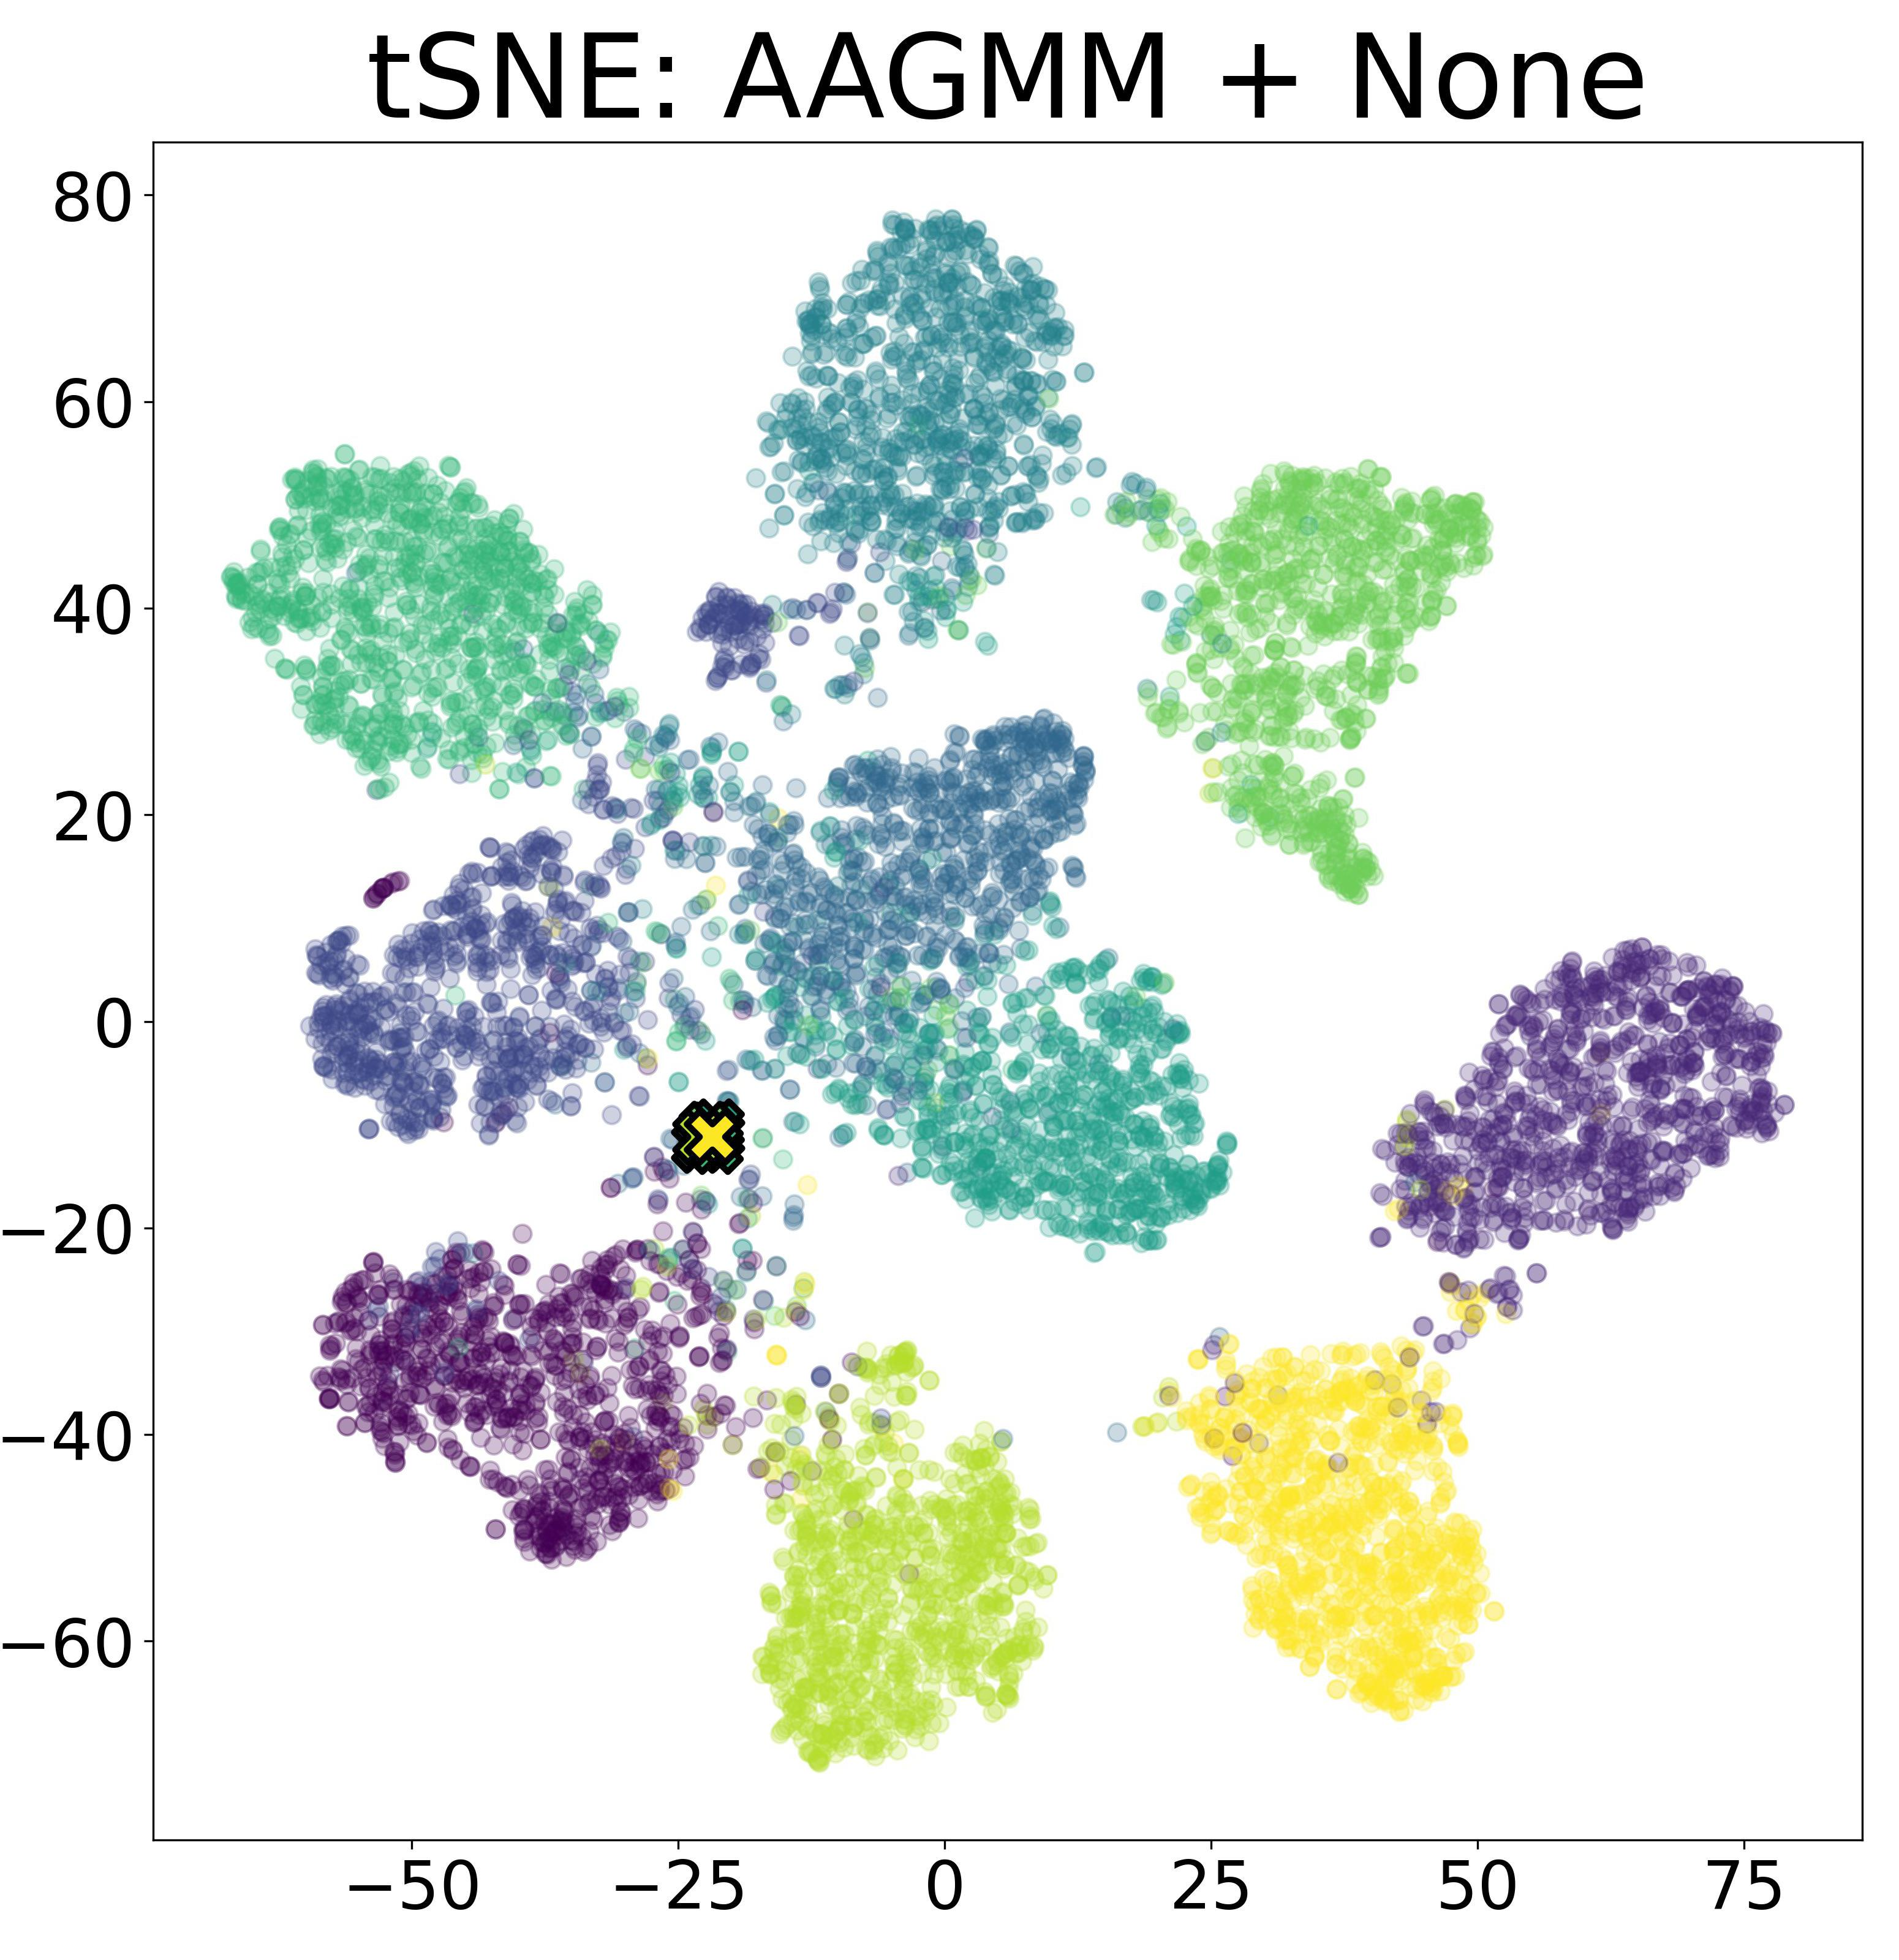
\includegraphics[width=.5\columnwidth]{figures/id-00000132-tsne.jpg}}
	\subfloat{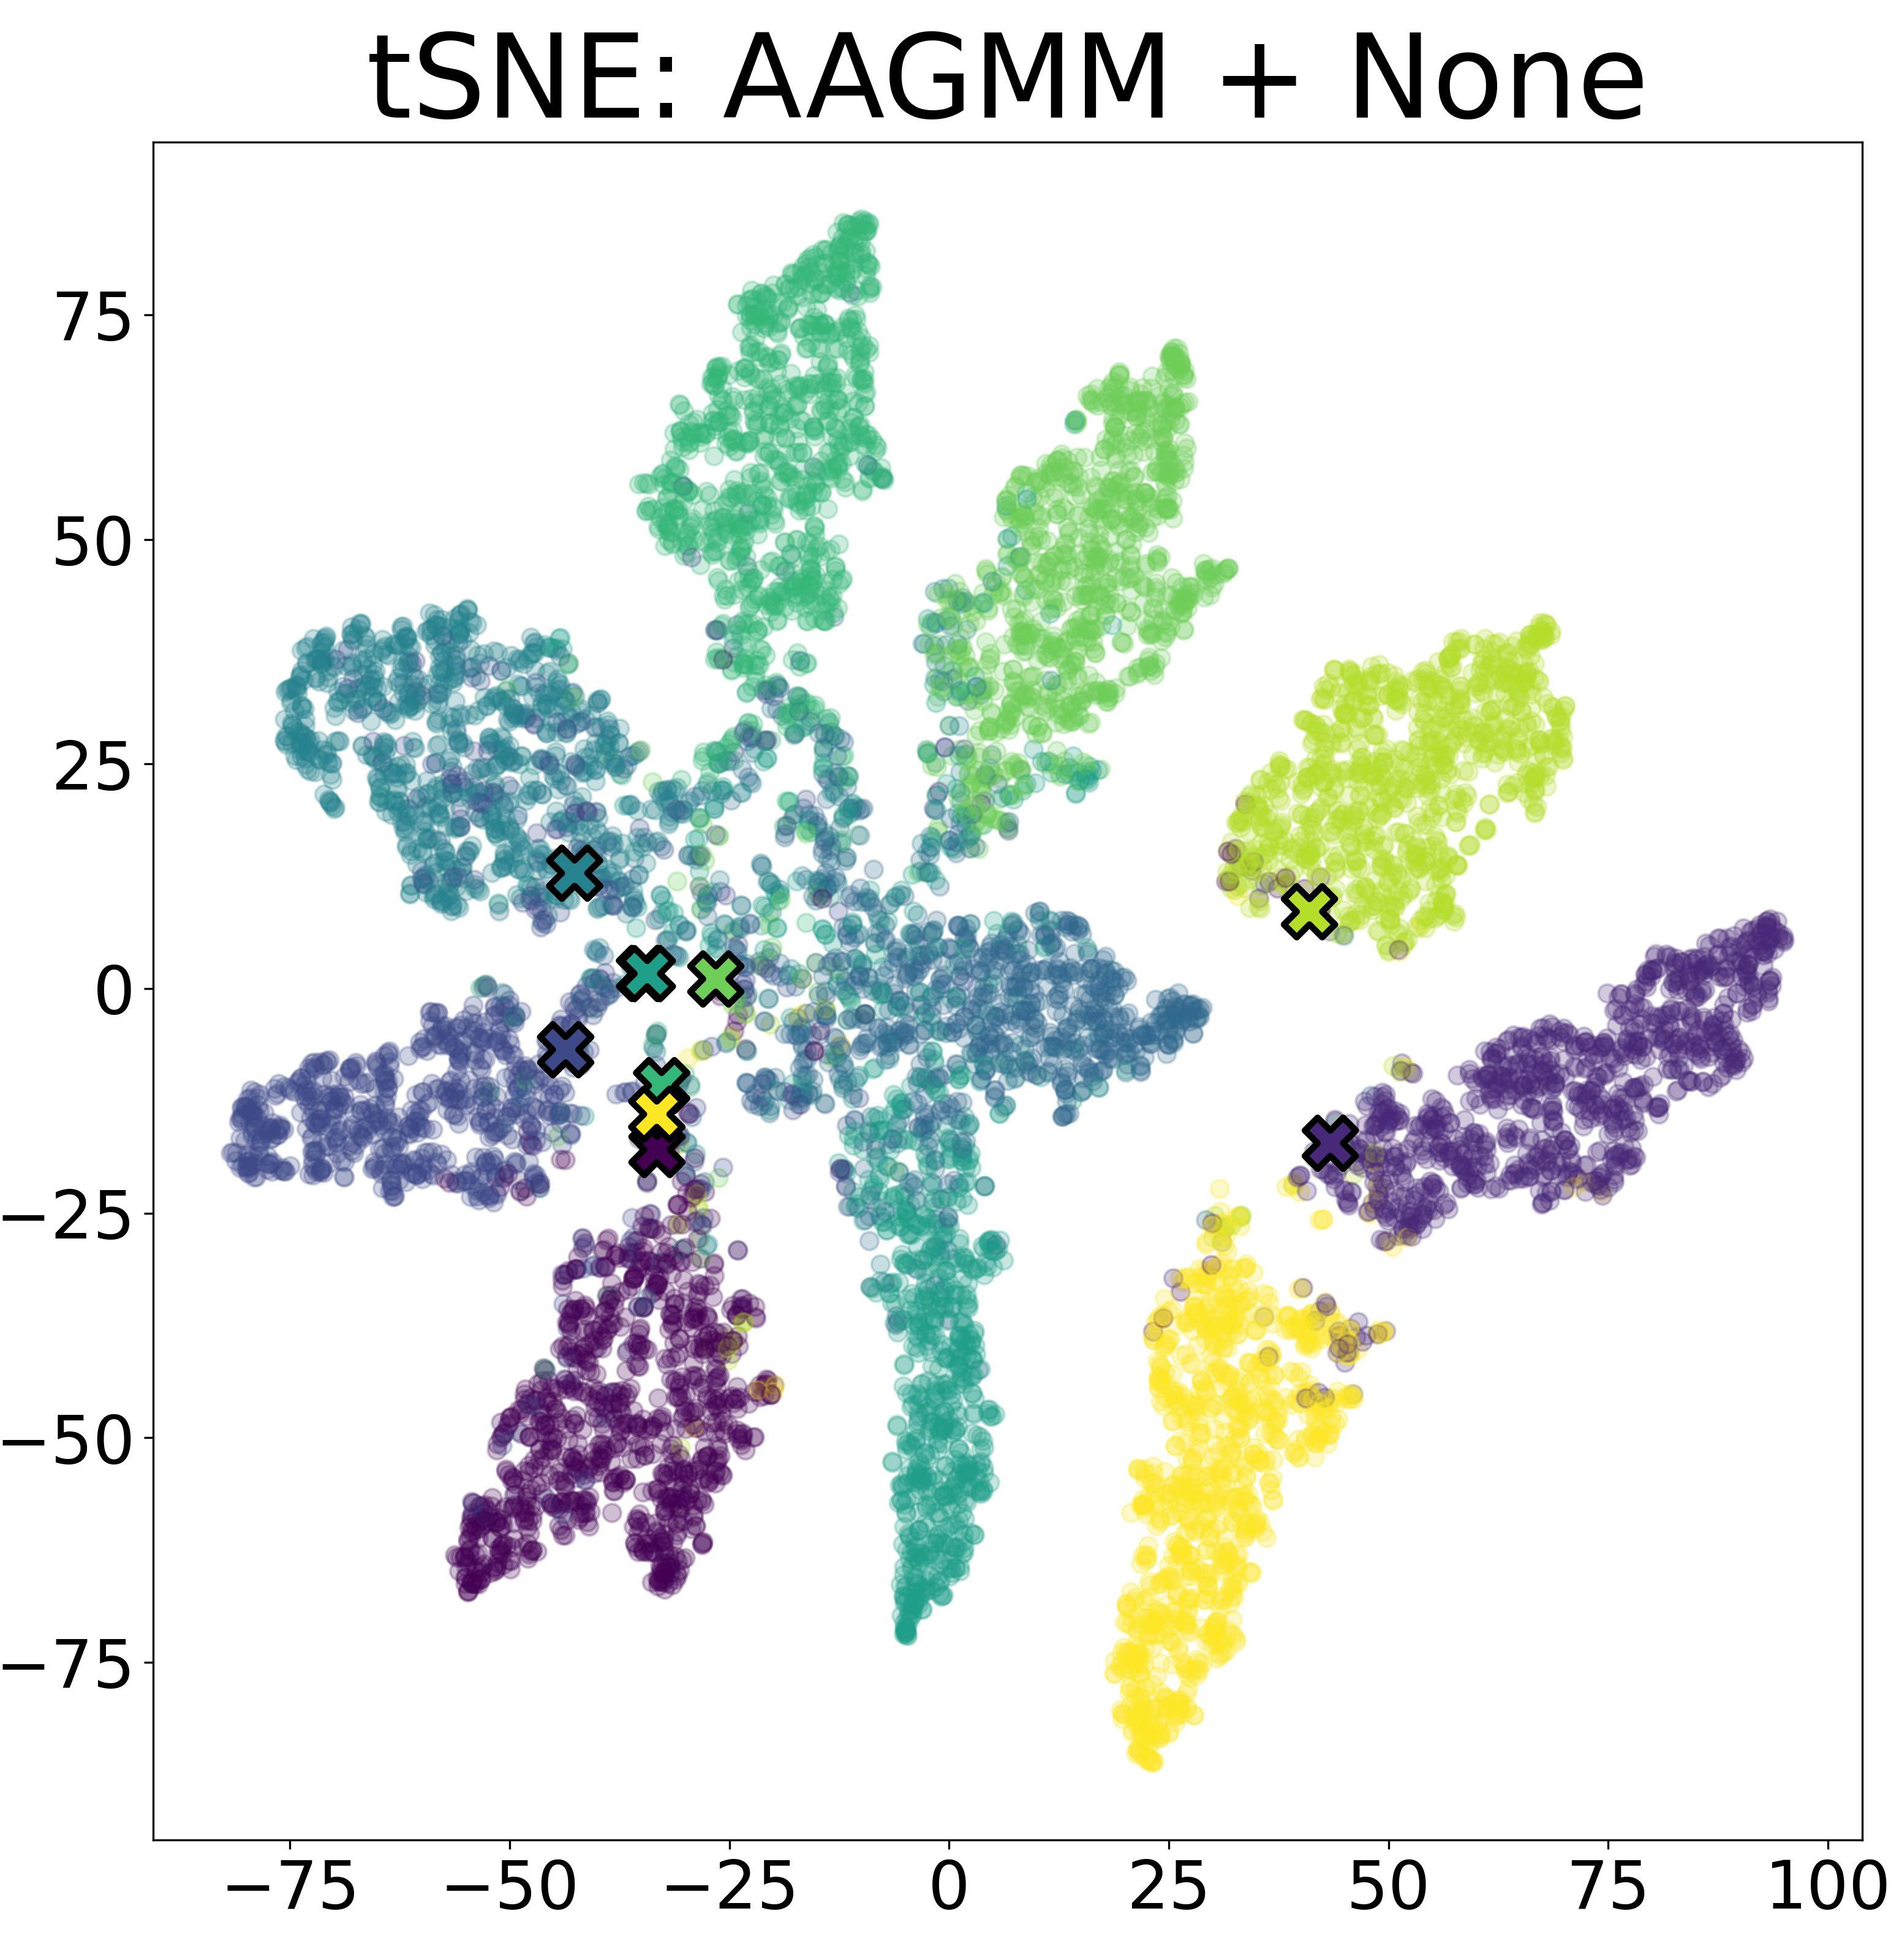
\includegraphics[width=.5\columnwidth]{figures/id-00000020-tsne.jpg}}
	\\
	\subfloat{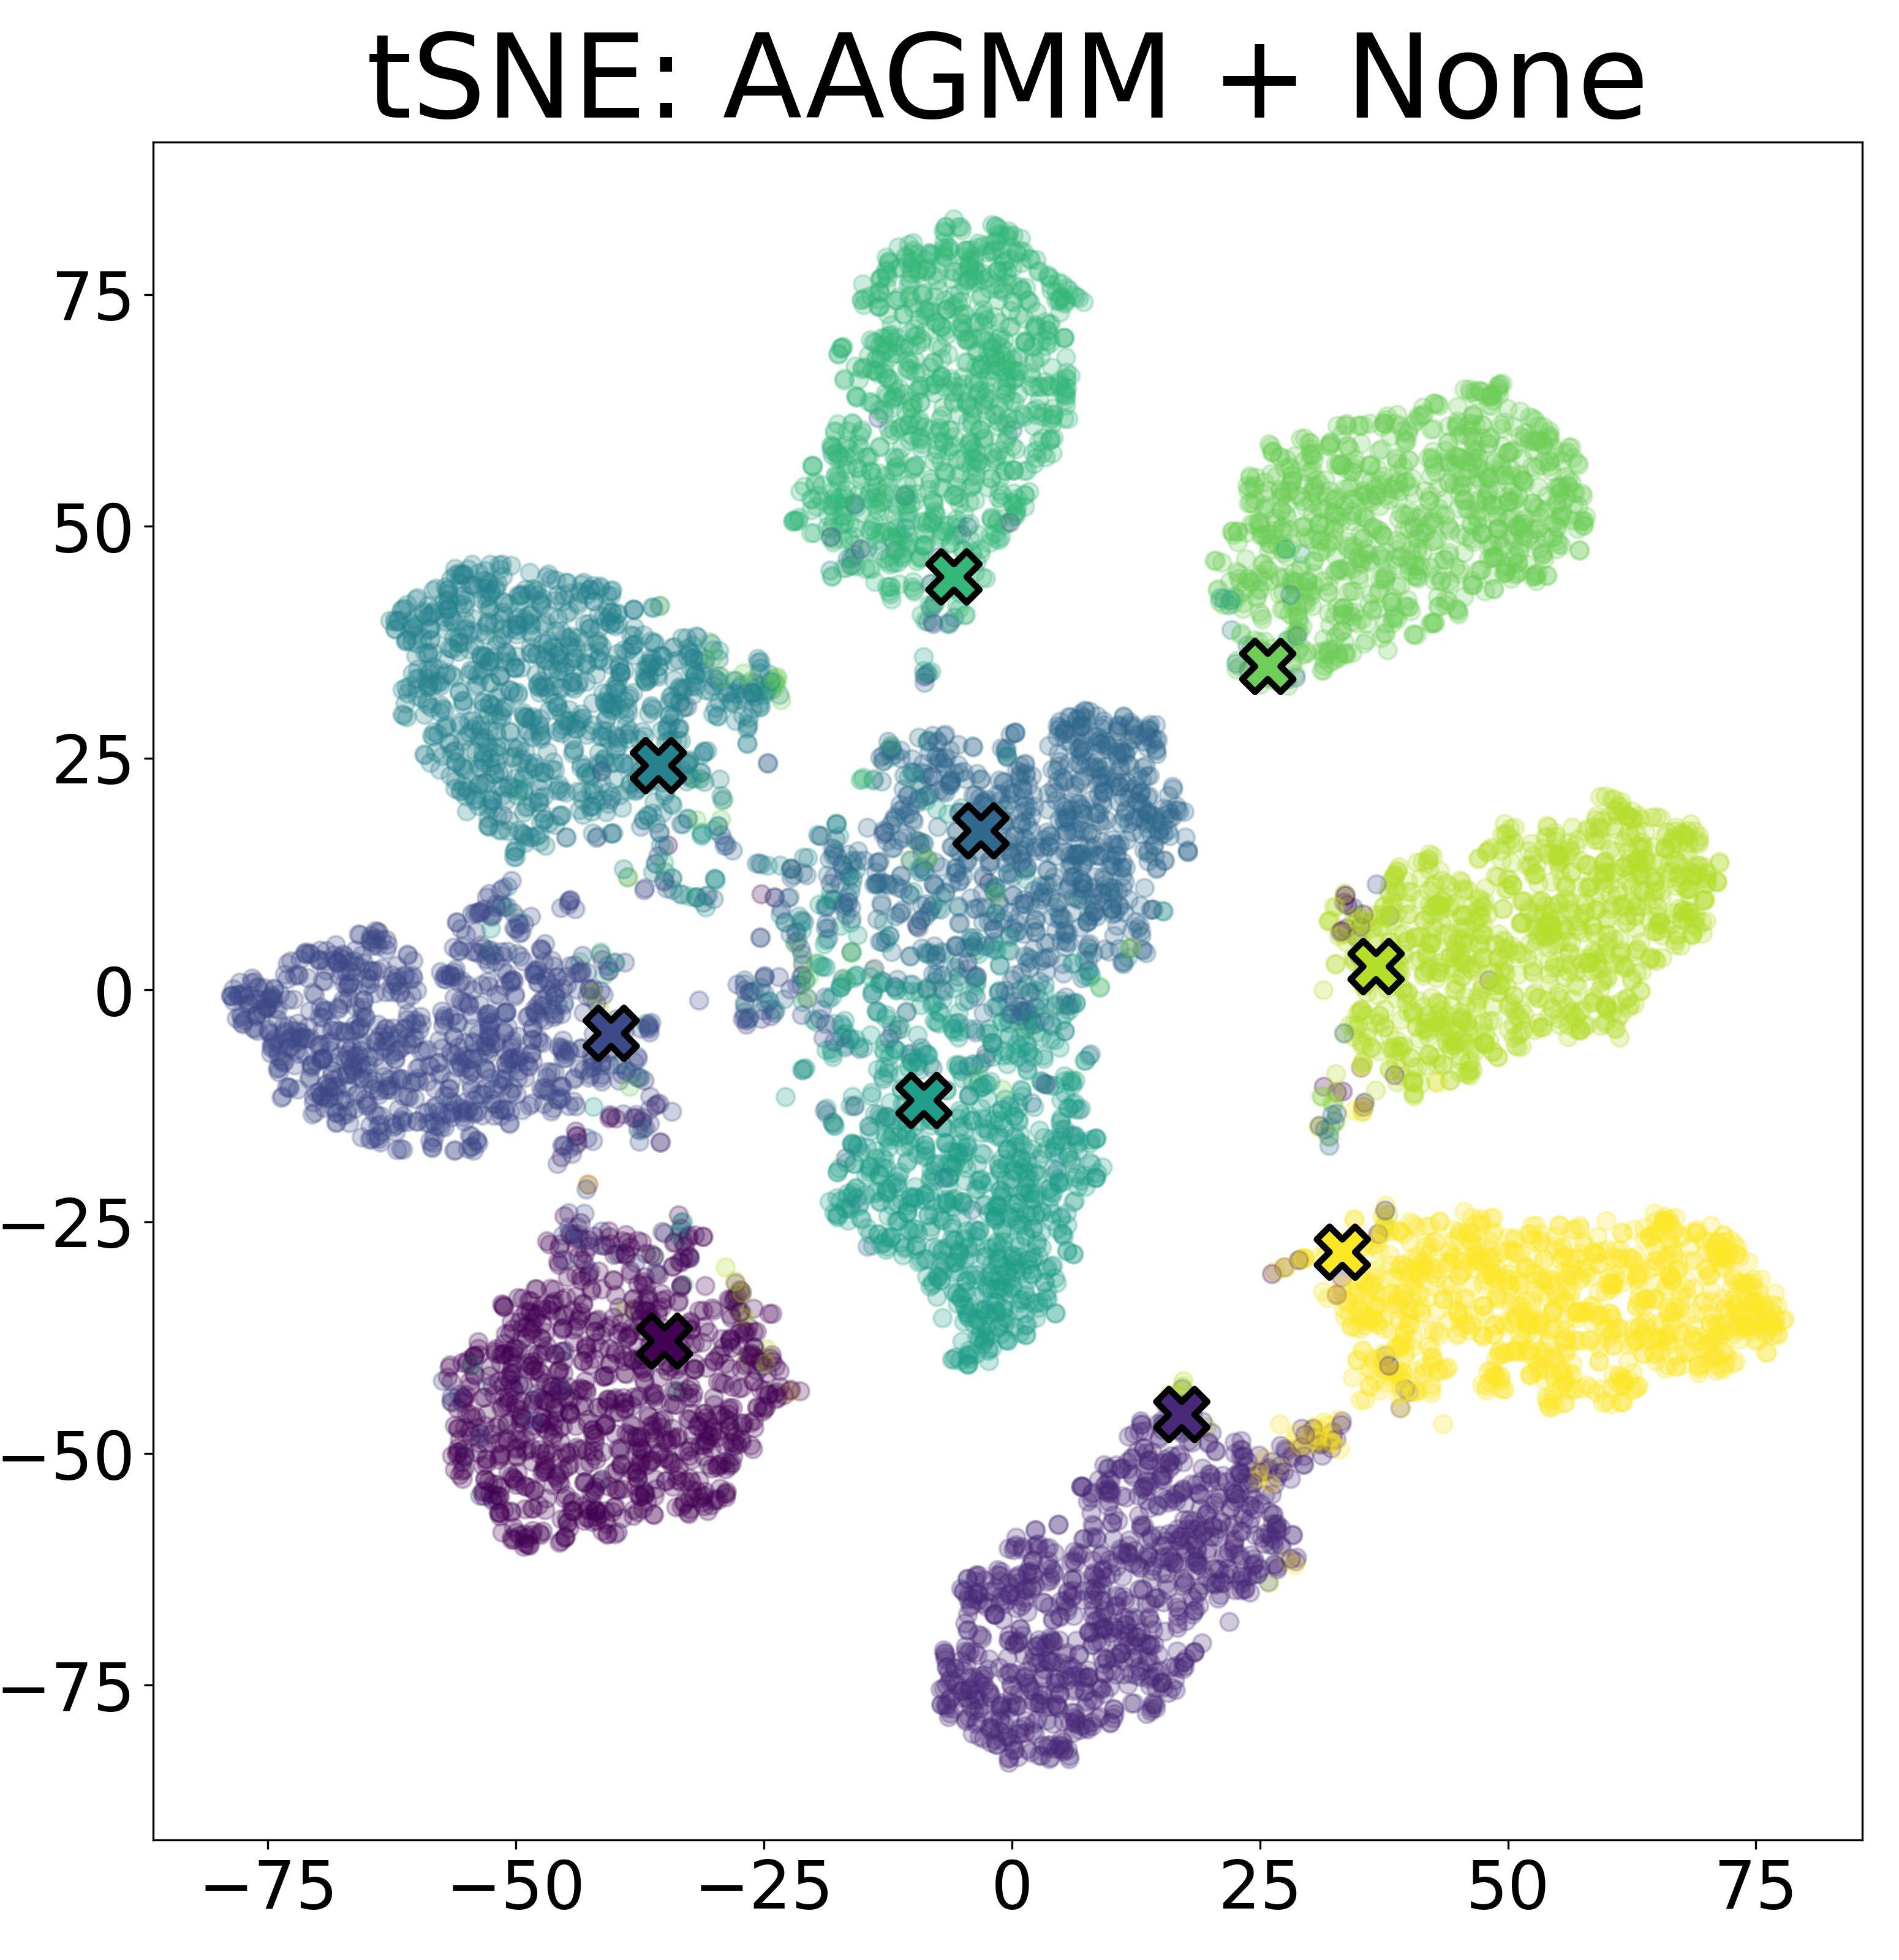
\includegraphics[width=.5\columnwidth]{figures/id-00000120-tsne.jpg}}
	\subfloat{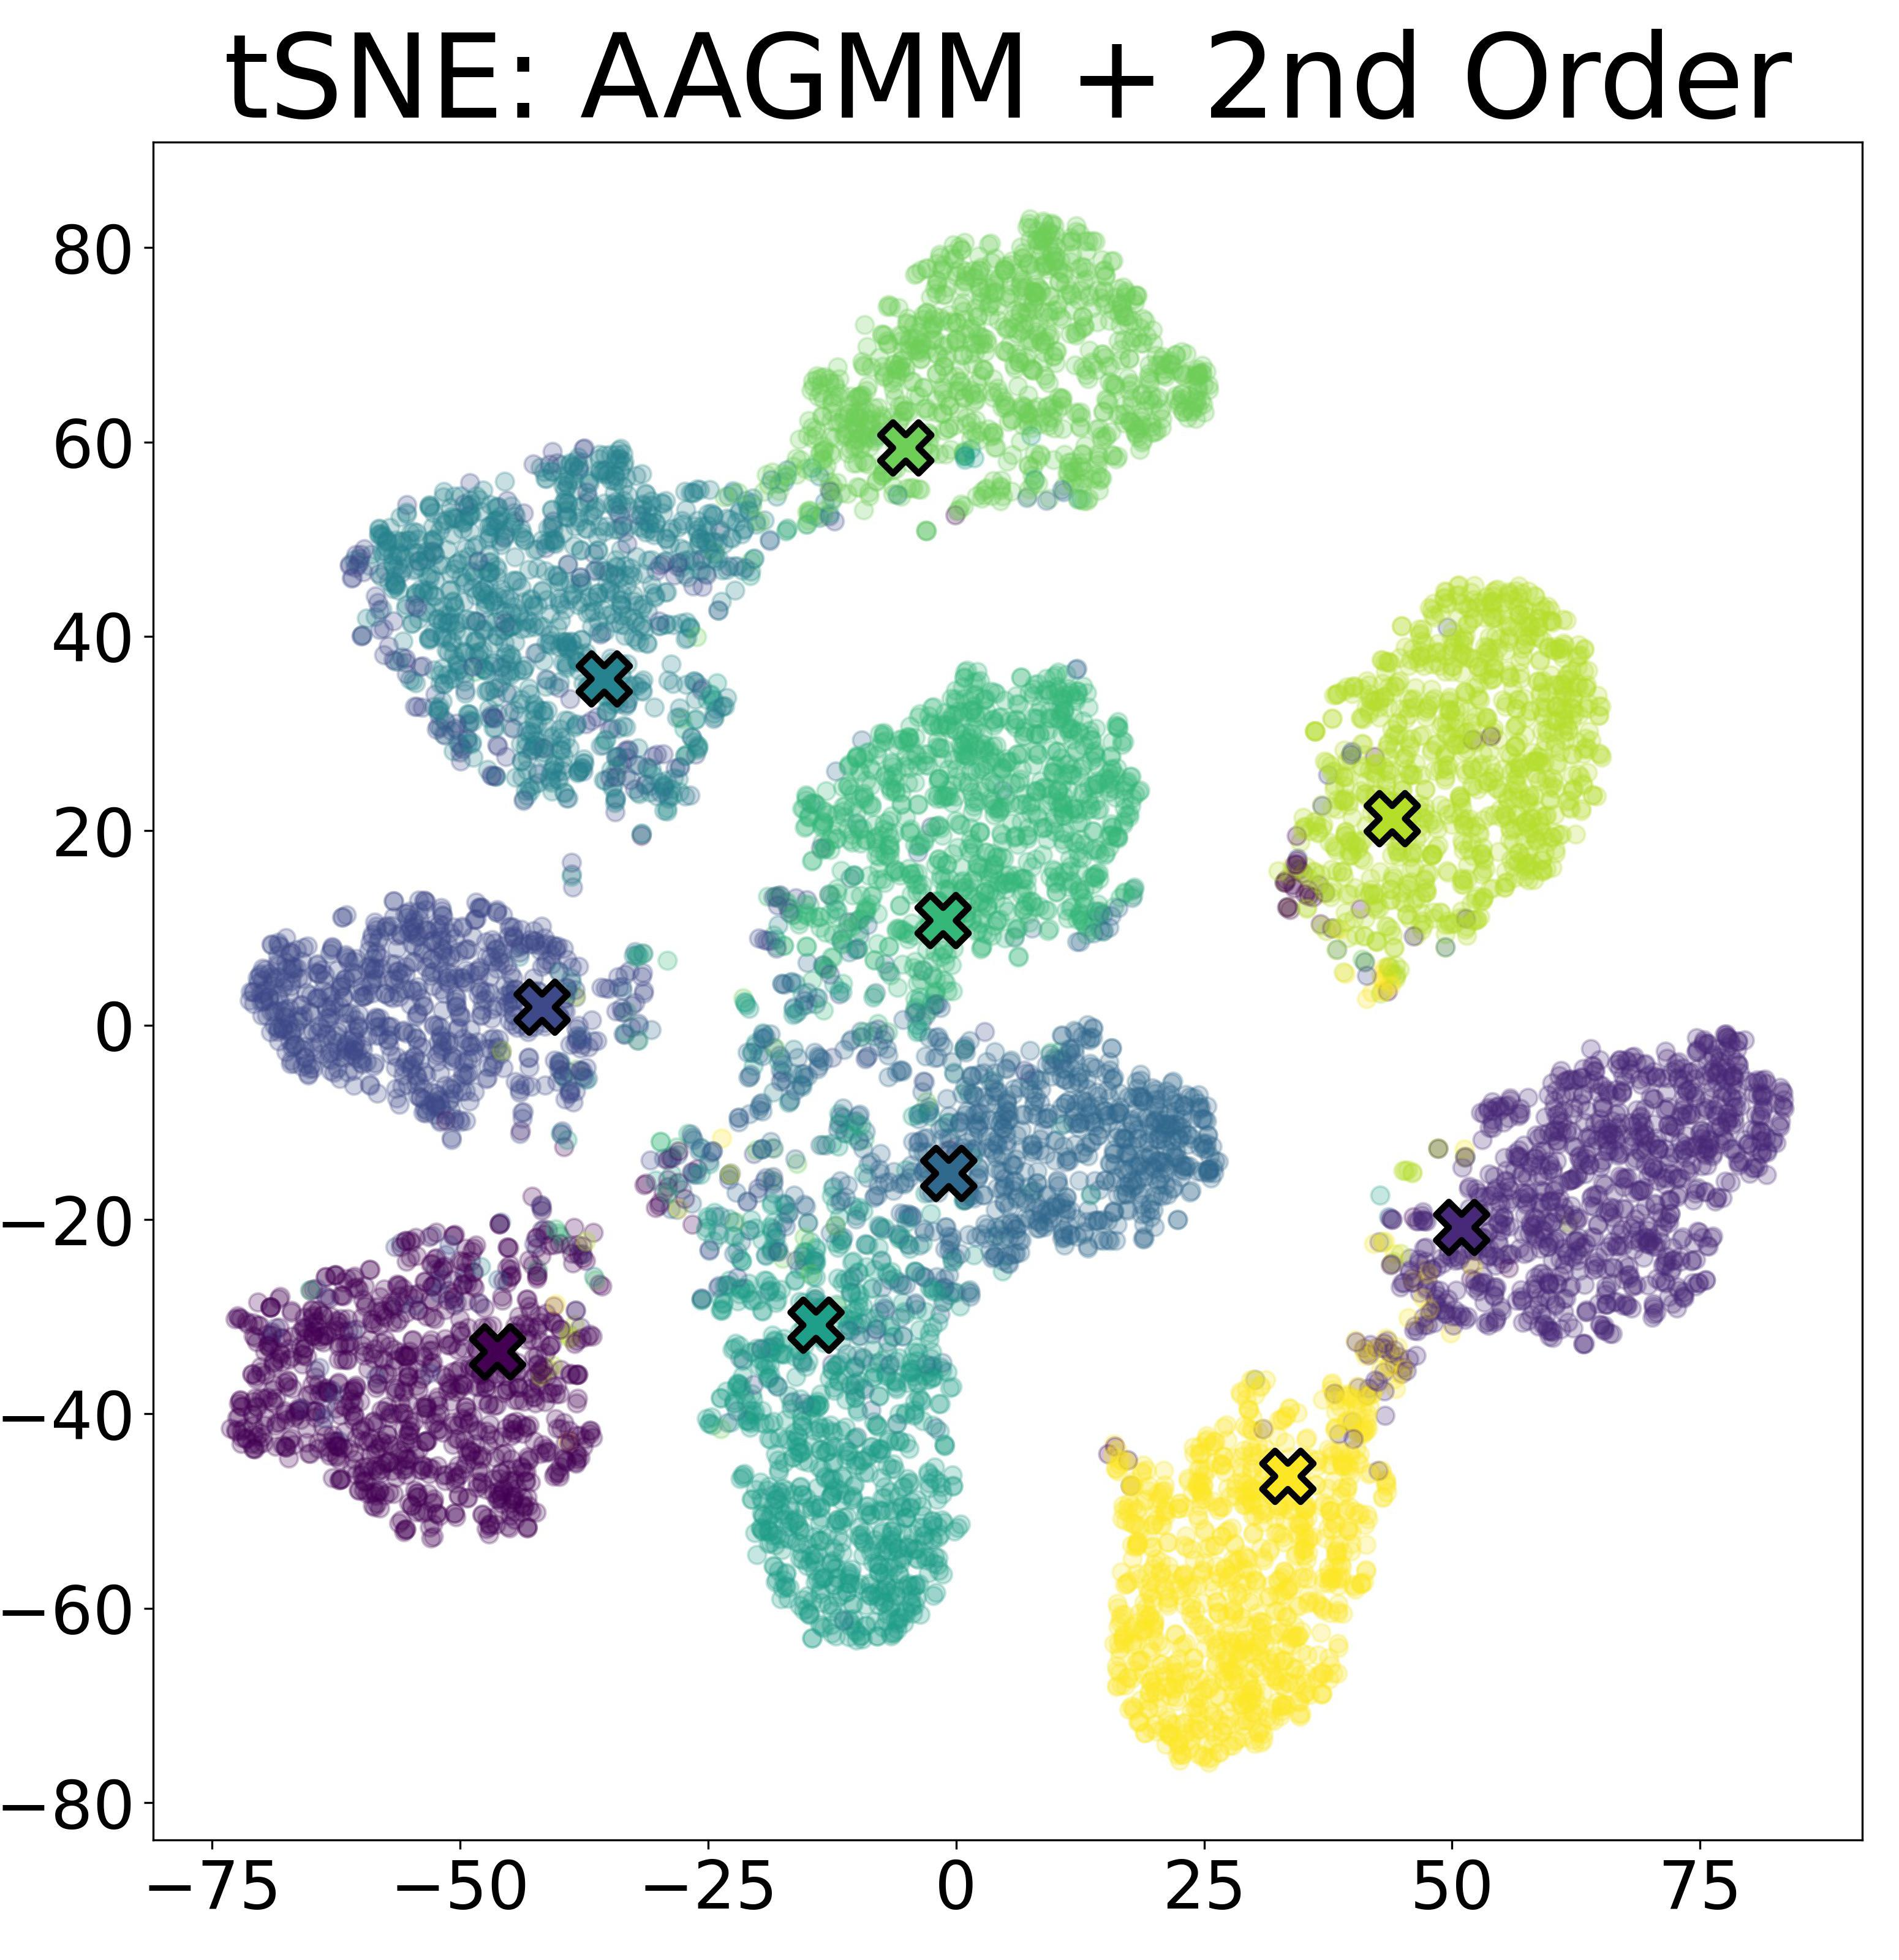
\includegraphics[width=.5\columnwidth]{figures/id-00000054-tsne.jpg}}
	
	%	\includegraphics[width=0.9\linewidth]{example-image-a}
	\caption{t-SNE plot of fully trained and reasonably accuracy AAGMM model's latent embedding space (with the learned cluster centers marked with X's). Depending on the run, the AAGMM cluster centers will be degenerate (top left), non-degenerate but still mis-aligned with the clusters (top right), acceptably aligned (bottom left), or well aligned with the underlying clusters when a 2nd order constraint is employed (bottom right).} 
	\label{fig:cifar10tsneaagmmnone}
\end{figure}




%\begin{table}[htbp]
%	\begin{tabular}{c|cc}
%		Method          & \multicolumn{2}{c}{CIFAR-10} \\ \hline
%		Label Count     & 40            & 250           \\
%		%Supervised & $77.18$ \scriptsize{$\pm1.32$}   & $56.24$ \scriptsize{$\pm3.41$}   \\ 
%		\hline
%		FixMatch\cite{sohn2020fixmatch}   & $13.81$ \scriptsize{$\pm3.37$}   & $5.07$ \scriptsize{$\pm0.65$}     \\
%		FlexMatch\cite{zhang2021flexmatch}  & $4.97$ \scriptsize{$\pm0.06$}    & $4.98$ \scriptsize{$\pm0.09$}    \\
%		FreeMatch\cite{wang2022freematch}  & $4.90$ \scriptsize{$\pm0.29$}    & $4.98$ \scriptsize{$\pm0.09$}    \\
%		SimMatchV2\cite{zheng2023simmatchv2} & $4.90$ \scriptsize{$\pm0.04$}    & $5.04$ \scriptsize{$\pm0.09$}    \\ \hline
%		Ours (AAGMM+None)    & $8.77$ \scriptsize{$\pm 2.89$}           & $5.91$ \scriptsize{$\pm 0.34$}  \\
%		Ours (KMeans+2ndOrder)    & $10.11$ \scriptsize{$\pm 2.79$}           & $6.84$ \scriptsize{$\pm 1.25$}  
%		
%	\end{tabular}
%	\caption{Error rate \% for CIFAR-10 SSL benchmark comparing to state of the art results. Results are copied from USB \cite{wang2022usb} unless otherwise stated. Existing results are drawn from FreeMatch\cite{wang2022freematch} and SimMatchV2\cite{zheng2023simmatchv2} publications.}
%	\label{table2}
%\end{table}



\section{Discussion}
% TODO fix conversational tone. Lots of opinion adjectives "only" "even"

\TODO{(chapman) need citation for VAE methods}
The most similar embedding constraint to our MoM as commonly seen in deep learning is the use of variational inference, as applied in Variational Auto-Encoder models (VAE).
VAE constrains the latent distribution using a KL-divergence penalty $D_KL(Q||P)$, where $Q(Z)$ is the variational distribution designed to approximate $p(Z|X)$, and $P$ is the target distribution, typically the multivariate standard normal distribution. 
Although the use of KL-divergence is strongly rooted in information theory, true calculation of KL-divergence is intractable, and thus approximations are often employed. 
% TODO make following sentence more quantitative/concrete
As such, the choice of the variational distribution $Q(Z)$ hides a great deal of error in approximation, limiting the VAE embedding constraint to penalize simple differences in the shape of the feature space.

In most VAE models the variational distribution $Q(Z)$ constrains the first order (mean) and second order diagonal moments (standard deviation).
Second order off-diagonal terms are usually discarded by VAE models.  
This means that most practical VAE models have no ability to constrain even the linear orthogonality of the feature space, because the cross-covariance terms are omitted to 'simplify' KL-divergence.  
By comparison, our MoM constraints not only constrain linearly orthogonality, but also penalize more complicated non-linear shape descriptions including skew, kutorsis, as well as complex multivariate hyper-covariance descriptions of shape.  
By penalizing higher order off-diagonal terms, we can produce feature spaces that are not only linearly orthogonal, but closely resemble true statistical independence.

One significant downside to our MoM embedding constraints is the exponential GPU memory requirements. 
The unreasonable amount of GPU memory required limits their practical application.
Additional optimization and/or avoiding the explicit creation of both the $nth$ order moment and its target value on device would likely improve the usability.

Semi-supervised learning is highly sensitive to both which samples are selected for the labeled population \cite{sohn2020fixmatch} and the stochasticity of the training process.
The stochasticity of training runs with the same starting seed (and identical labeled samples) will quickly diverge due to the randomness inherent in the training process.
Anecdotally its worse in semi-supervised than fully supervised.
To characterize this variance, and hence how much we should trust the error bars for our 5 runs, we took a few of our configurations and ran them $N=5$ times with the same seed with CIFAR-10 at 40 labeled samples.
This produced the potentially widely varying final model accuracies seen in Table \ref{tab:runseedvariability}.

\begin{table}[h!]
	\begin{tabular}{r|c|c|c|c}
		\multicolumn{5}{c}{Identical Seed Runs on CIFAR-10 at 40 Labels}\\
		\hline
		 & \small{\makecell{AAGMM\\+2nd Order}} & \small{\makecell{KMeans\\+2nd Order}} & \small{\makecell{AAGMM\\+None}} & \small{\makecell{KMeans\\+None}} \\
		\hline
		Run 1 & $87.5$ & $86.9$ & $71.2$ & $xx.y$ \\
		Run 2 & $85.6$ & $91.2$ & $67.9$ & $xx.y$ \\
		Run 3 & $84.8$ & $77.7$ & $xx.y$ & $xx.y$ \\
		Run 4 & $85.3$ & $87.6$ & $xx.y$ & $xx.y$ \\
		Run 5 & $85.2$ & $xx.y$ & $xx.y$ & $xx.y$ \\
	\end{tabular}
	\caption{Test accuracy for independent training runs with the same random seed for various final layer configurations. All runs use the 128D (default) model latent embedding. All runs use the same labeled samples. \TODO{(majurski) update table with final few currently running experiments}}
	\label{tab:runseedvariability}
\end{table}

Future work in this area should explore both accuracy improvements as well as implementation optimization to ensure the novel final layers are not prohibitively memory expensive to use.
Additionally, one should explore how to best take advantage of the better behaved latent embedding space to improve data efficiency for model training. 

We demonstrate a fully differentiable Axis-Aligned Gaussian Mixture Model with Method of Moments based latent embedding space constraints to improve the generative inlier/outlier performance of image classification deep learning models. 
This preliminary work constructs those novel layers with the associated constraints, and demonstrates reasonable performance on challenging benchmark semi-supervised learning tasks.



{
	\small
	\bibliographystyle{ieeenat_fullname}
	\bibliography{refs}
}


\end{document}